% final draft
% todo: Interkapitel-Referenzen, Kontextgrafik

\chapter{Articulation Work} % (fold)
\label{cha:articulation_work}

In diesem Kapitel wird das Konzept „Articulation Work“ dargestellt und in den Kontext von menschlicher Arbeit gestellt. Der erste Teil geht auf die historische Entwicklung des Begriffs „Articulation Work“ und die unterschiedlichen Herangehensweisen zu dessen Verständnis ein. Der zweite Teil des Kapitels widmet sich den Aktivitäten, die im Rahmen von „Articulation Work“ durchgeführt werden, den Merkmalen, an denen sich effektive „Articulation Work“ zeigt, sowie den Möglichkeiten der Unterstützung von „Articulation Work“ durch organisationale und technische Maßnahmen. Abbildung \ref{fig:img_Kontextgrafiken_k2} stellt dieses Kapitel und dessen Aufbau im Kontext der anderen inhaltlich vor- und nachgelagerten Kapitel dar.


\begin{figure}[htbp]
	\centering
		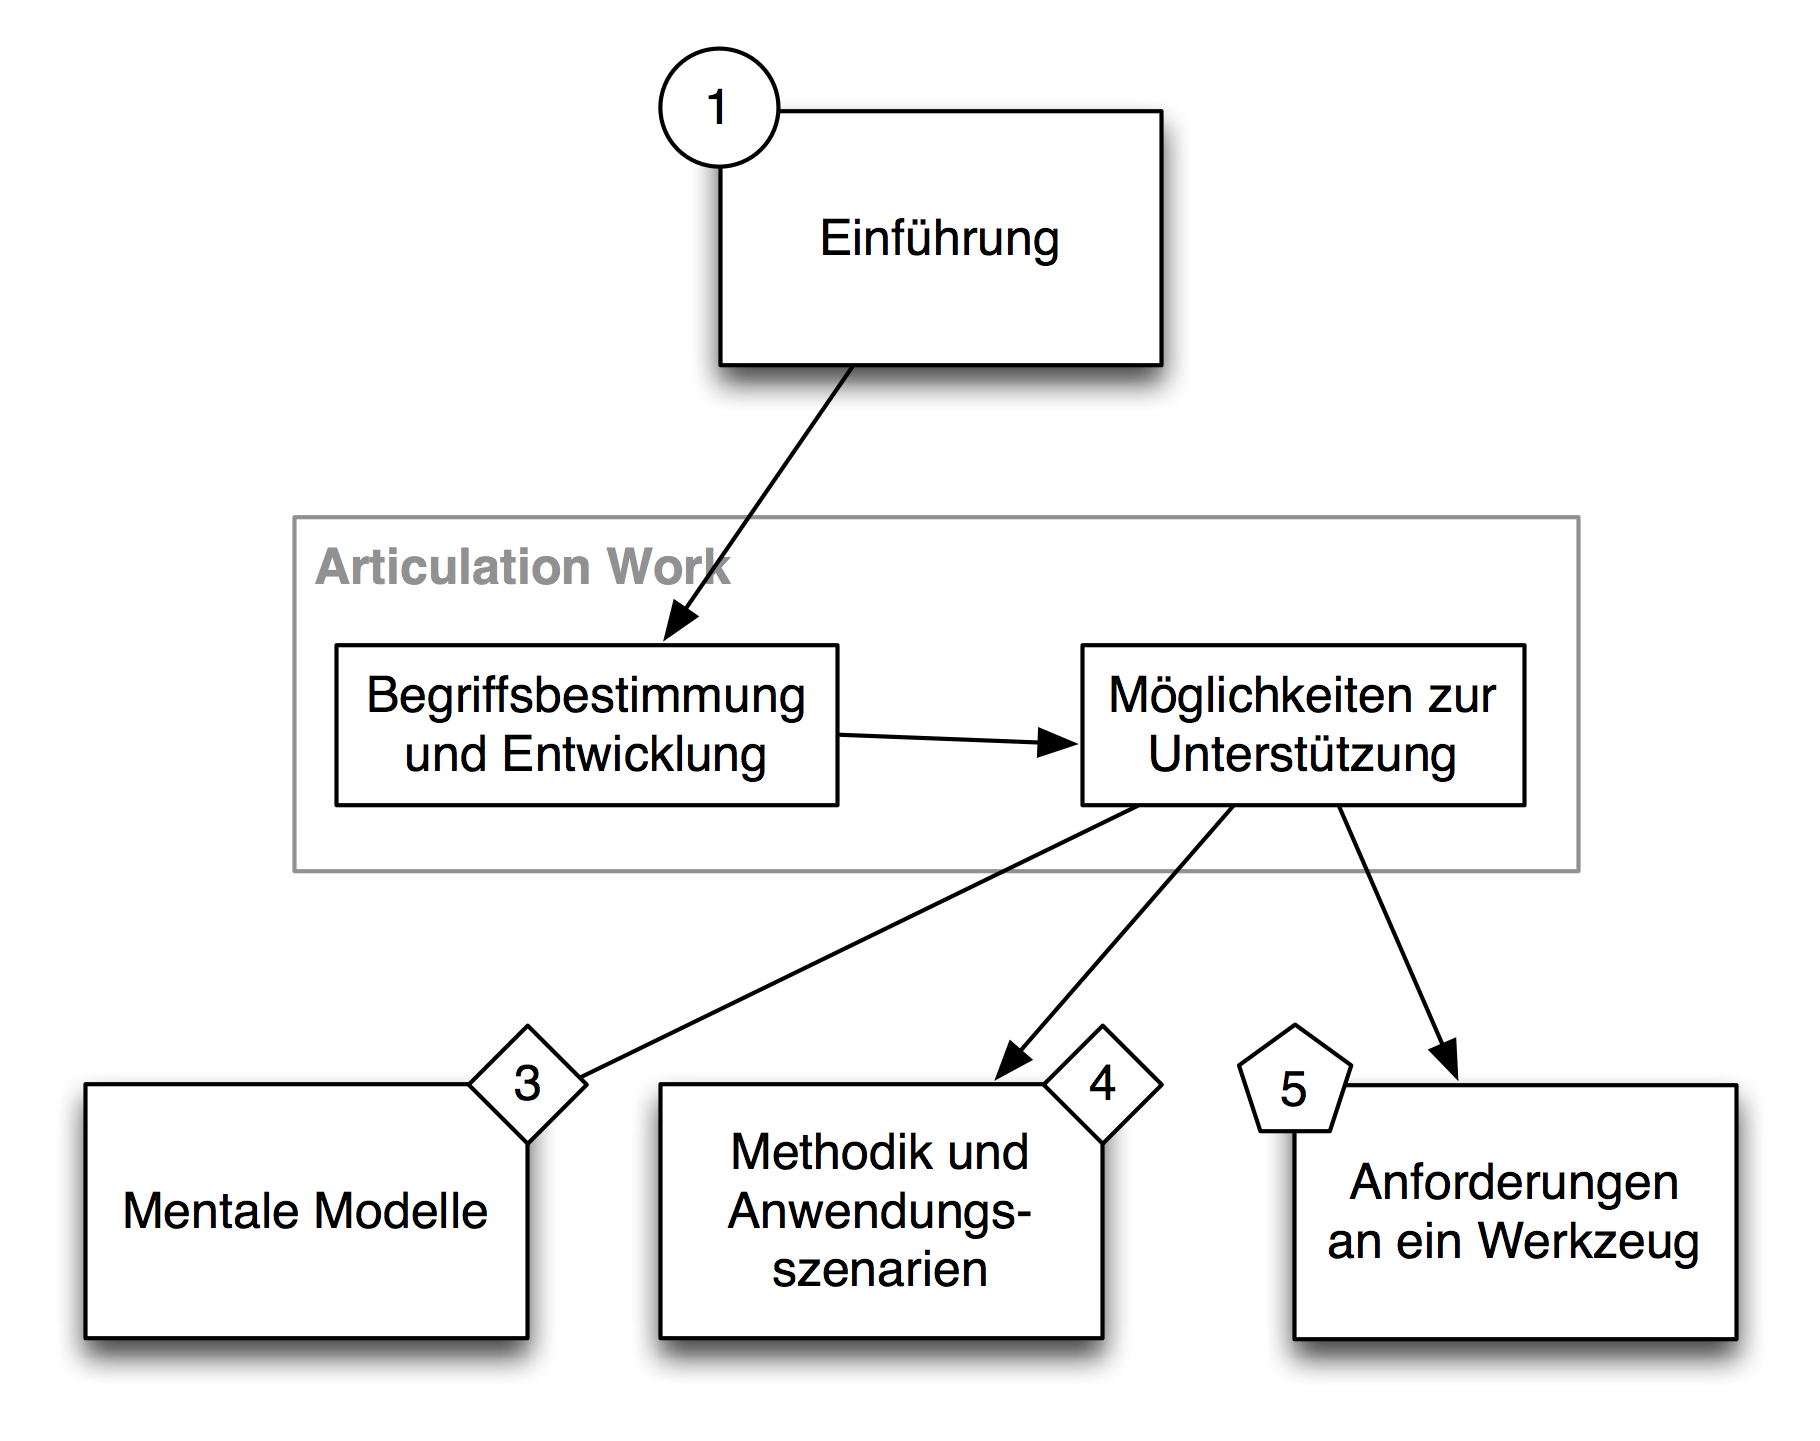
\includegraphics[scale=0.6]{img/Kontextgrafiken/k2.png}
	\caption{Kapitel „Articulation Work“ im Gesamtzusammenhang}
	\label{fig:img_Kontextgrafiken_k2}
\end{figure}

\section{Begriffsbestimmung} % (fold)
\label{sec:aw_begriffsbestimmung}

Das Konzept „Articulation Work“ wurde als Erklärungsmodell für eine bestimmte Art von menschlicher Arbeit Mitte der 1980er Jahre von \citet{Strauss85} eingeführt. Neben \citet{Strauss85} tragen auch die Arbeiten von \citet{Gerson86} und \citet{Fujimura87} wesentlich zur Begriffsbestimmung und Konzeptbildung bei. Die vorhandene Literatur, die Bezug auf „Articulation Work“ nimmt (siehe Anhang \ref{cha:literatur_zum_themengebiet_articulation_work}), referenziert im Wesentlichen auf eine oder mehrere dieser drei Arbeiten. Der Kontext, in dem die Entwicklung der im Folgenden vorgestellten Konzepte erfolgte, war die komplexe, von viel Interaktion an zahlreichen Schnittstellen geprägte Arbeit in Krankenhäusern \citep{Strauss85}, in der Wissenschaft \citep{Fujimura87} und in Versicherungsunternehmen \citep{Gerson86}, die die jeweiligen Autoren in mehreren Fallstudien untersuchten. 

Um in der Folge einen einheitlichen Begriffsraum aufspannen zu können, ist vorab der Begriff „Arbeit“ zu klären. Die eben genannten Autoren führen keine explizite Definition an, weshalb hier auf eine Definition zurückgegriffen wird, die im Kontext der folgenden Ausführungen zur „inneren“ Struktur von Arbeit nach „außen“ hinreichend umfassend ist\footnote{Auf eine umfassende Literaturstudie und die Entwicklung eines darauf aufbauenden „Arbeits“-Begriffs wurde hier verzichtet, da dies über den Betrachtungsbereich und Anspruch dieser Arbeit hinausgeht}. \citet{Semmer04} definieren vor dem Hintergrund der Organisationspsychologie „Arbeit“ wie folgt: 

\emph{„Arbeit ist zielgerichtete menschliche Tätigkeit zum Zwecke der Transformation und Aneignung der Umwelt aufgrund selbst- oder fremddefinierter Aufgaben, mit gesellschaftlicher, materieller oder ideeller Bewertung, zur Realisierung oder Weiterentwicklung individueller oder kollektiver Bedürfnisse, Ansprüche und Kompetenzen.“} 

Arbeit ist also ein menschliches Phänomen, Träger von Arbeit sind immer Menschen. Arbeit definiert sich außerdem durch ihre Zielgerichtetheit und findet immer in Interaktion mit der Umwelt statt. Die Ziele, auf die Arbeit ausgerichtet ist, leiten sich aus Aufgaben ab, die sich Menschen selbst setzten können oder die ihnen vorgegeben werden. Diese Aufgaben dienen der Erreichung von individuellen oder kollektiven Bedürfnissen und Ansprüchen bzw. der (Weiter-)Entwicklung von Kompetenzen. Die Bewertung der Zielerreichung muss nicht unbedingt aus materieller Perspektive erfolgen sondern kann auch ideell oder gesellschaftlich begründet sein. 

In dieser Arbeit wird der Begriff „Arbeit“ vor allem auch im organisationalen Kontext gesehen. Ein wesentlicher Aspekt ist in diesem Zusammenhang die Arbeitsteilung, also die koordinierte Tätigkeit mehrerer Individuen um ein gemeinsames Ziel zu erreichen. Dies stellt die obige Definition nicht in Frage \citep{Schmidt94}, erweitert jedoch den Betrachtungsbereich explizit auch auf Arbeit, die gemeinschaftlich durchgeführt wird\footnote{\emph{„[\ldots] work is an individual phenomenon in so far as labor power happens to be tied to individuals and cannot be separated from the individuals. That is, a cooperative work process, is performed by individuals with individual interests and motives.“}\citep[][S. 353]{Schmidt94}}. 

„Articulation Work“ ist jener Anteil der gesamten durchgeführten Arbeit, der der Abstimmung mit anderen Individuen dient. Diese Abstimmung ist notwendig, um das eigentliche Arbeitsziel erreichen zu können. Arbeit wird von den oben angeführten Autoren als inhärent kooperativer Prozess gesehen, der immer auf Interaktion mit anderen Menschen basiert bzw. diese bedingt (Strauss formuliert diese Annahme in Bezugnahme auf \citet{Hughes71} prägnant mit der Aussage \emph{„work rests ultimately on interaction“}). Diese Annahme erscheint insofern als zulässig, als dass selbst Arbeitsabläufe, die selbst keine Kooperation mit anderen Menschen mit sich bringen, zumindest auf den Ergebnissen anderer Arbeitsabläufe aufbauen oder als Grundlage weiterer Arbeitsabläufe dienen. Interaktion tritt also in jedem Arbeitsprozess zumindest zu Beginn und am Ende in unmittelbarer oder mittelbarer\footnote{Unter „mittelbar“ ist hier Interaktion zu verstehen, die nicht im direkten Kontakt zwischen Individuen abläuft, sondern lediglich indirekt durch die Ergebnisse eines Arbeitsprozesses (Materialien, Dokumente, \ldots) vermittelt wird.} Form auf. Diese Annahme wird  auch von \citet{Schmidt94} unterstützt, der darauf hinweist, dass individuelle Arbeit und kooperative Arbeit oft nicht klar abgrenzbar sind bzw. dynamisch ineinander übergehen\footnote{\emph{„Cooperative work and individual work should not be conceived of as different work domains. In daily work practice, cooperative and individual activities are inextricably interwoven. [\ldots] More than that, the boundary between individual and cooperative work is dynamic in the sense that people enter into cooperative work relations and leave them according to the requirements of the current situation and the technical and human resources at hand.“}\citep[][S. 352]{Schmidt94}}.

Jener Teil von Arbeit, der der eigentlichen Zielerreichung dient, wird im hier vorgestellten Erklärungsmodell als „Production Work“ bezeichnet \citep{Fujimura87}. „Production Work“ ist komplementär zu „Articulation Work“ zu sehen und umfasst alle Aktivitäten, die der „Wertschöpfung“ im wörtlichen Sinn dienen. „Production Work“ sind also alle Tätigkeiten, die mit der Schaffung jener Werte (oder Ergebnisse) befasst sind, die durch den Arbeitsablauf erreicht werden sollen.  

\begin{figure}[htbp]
	\centering
		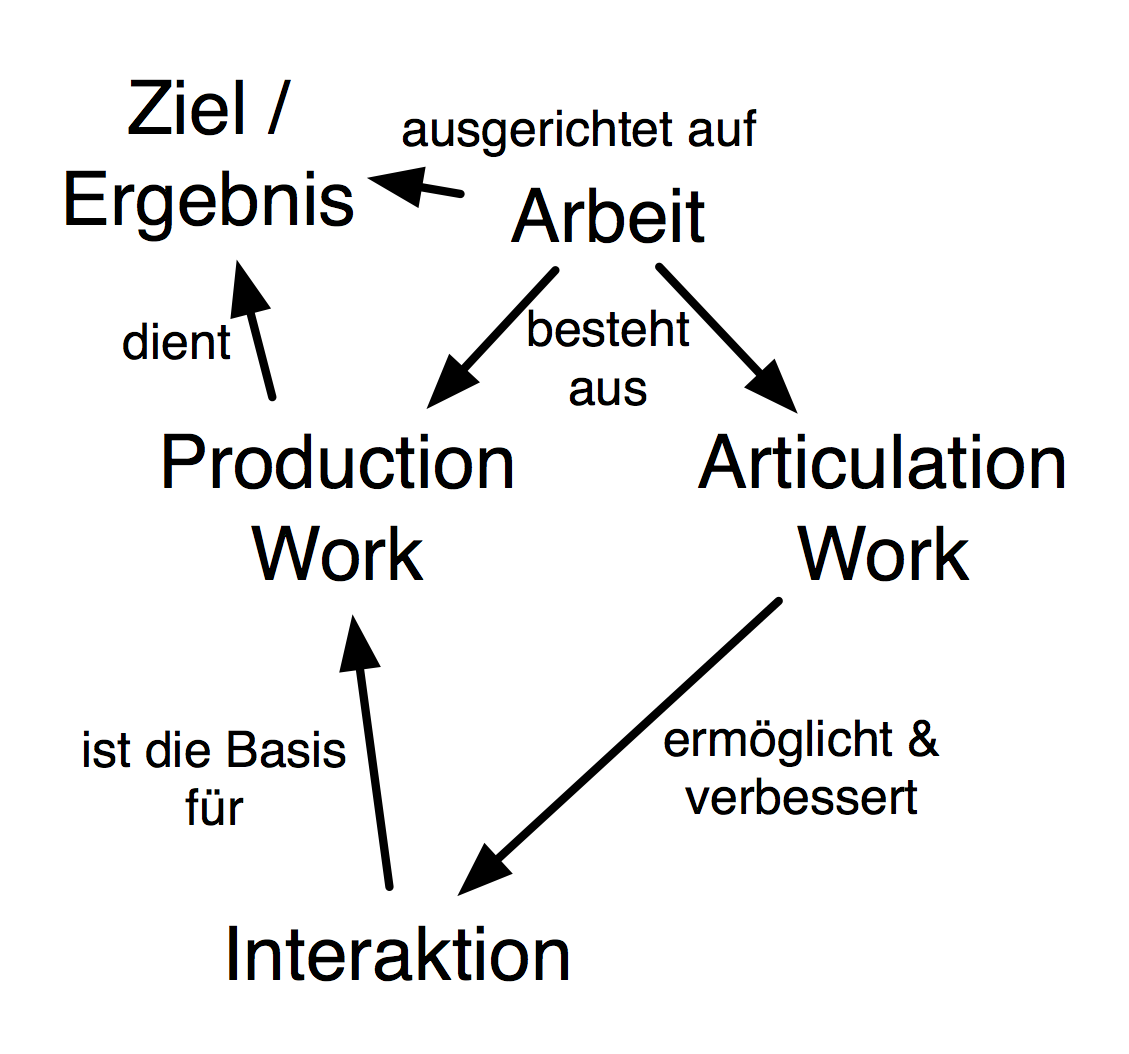
\includegraphics[width=5cm]{img/ArticulationWork/ArbeitInteraktion.png}
	\caption{Konzeptualisierung von Arbeitsabläufen}
	\label{fig:img_ArticulationWork_ArbeitInteraktion}
\end{figure}

Teile eines Arbeitsablaufs dienen also der Zielerreichung an sich („Production Work“). Andere Teile dienen der Abstimmung zwischen den involvierten Akteuren, um ein gemeinsames Verständnis über die jeweiligen Schnittstellen -- also die Berührungspunkte zwischen den Tätigkeiten -- zu entwickeln (siehe Abbildung \ref{fig:img_ArticulationWork_ArbeitInteraktion}). Diese Entwicklung eines gemeinsamen Verständnisses bzw. diese „Koordination“ ist kritisch für den Erfolg von kooperativer Arbeit \citep{Strauss93} und wird als „Articulation Work“ bezeichnet.\footnote{\emph{„Since the plurality of tasks making up their totality, as well as the relations of actors to tasks, are not automatically articulated, actors must do that too, and often in complex ways. We call the work of doing this "articulation work" -- a supra-type of work.“}\citep{Strauss85}} 

„Articulation Work“ ermöglicht also funktionierende Kommunikation und Zusammenarbeit im eigentlichen Arbeitsablauf. Zentral ist dabei vor allem die gegenseitigen Offenlegung der Annahmen aller beteiligten Personen, die den individuellen Arbeitsbeiträgen zugrunde liegen\footnote{\emph{„Reconciling incommensurate assumptions and procedures in the absence of enforceable standards is the essence of articulation.“}\citep[][S. 266]{Gerson86}}. 

„Articulation Work“ ist keine Tätigkeit, die zu einem bestimmten Zeitpunkt im Arbeitsprozess durchgeführt wird und dann als abgeschlossen betrachtet werden kann\footnote{\emph{„The articulation work involves the pre-articulation of the tasks, their management and post-articulation.“}\citep[][S. 121]{Raposo04}}. Vielmehr wird „Articulation Work“ immer auch begleitend zur eigentlichen produktiven Arbeit durchgeführt und umfasst neben planenden und koordinierenden Tätigkeiten auch das Erkennen von Fehlentwicklungen bzw. von Situationen, in denen eine erneute Koordination notwendig ist\footnote{\emph{„Articulation consists of all the tasks involved in assembling, scheduling, monitoring, and coordinating all of the steps necessary to complete a production task.“}\citep[][S. 266]{Gerson86}}. 

Der Begriff „Articulation Work“ ist im Englischen zweideutig und von \citeauthor{Strauss85} auch bewusst so gewählt. Einerseits wird damit ausgedrückt, dass \emph{Arbeit} („Work“) artikuliert wird, andererseits zeigt der Begriff, das die \emph{Artikulation} selbst ebenfalls Arbeit ist (also Zeit und Ressourcen in Anspruch nimmt) und auch also solche wertgeschätzt werden muss \citep{Fujimura87}. Gleichzeitig kennzeichnet er auch die rekursive Natur von „Articulation Work“, die somit jederzeit selbst Gegenstand von „Articulation Work“ werden kann \citep{Star99}. „Articulation Work“ ist kein klar abgegrenztes und strukturiertes Konzept -- sie tritt je nach Arbeitssituation in unterschiedlichen Spielarten auf. Die Unterscheidung dieser Arten von „Articulation Work“ ist für die Unterstützung derselben relevant und wird daher im folgenden Abschnitt genauer betrachtet.
% section begriffsbestimmung (end)

\section{Ausprägungen von Articulation Work} % (fold)
\label{sec:arten_von_articulation_work}

Wie bereits von \citet{Gerson86} angeführt, argumentiert auch \citeauthor{Strauss88}, dass Artikulation immer passieren muss (und passiert), wo Menschen zusammenarbeiten, um zu vermeiden, dass unbekannte Aspekte Probleme bei der Durchführung der Arbeit verursachen \citep{Strauss88}. „Articulation Work“ ist kein revolutionäres Konzept, sondern fasst Tätigkeiten unter einem Begriff zusammen, die seit jeher Teil jeder Zusammenarbeit zwischen Menschen sind \citep{Strauss88}. Grundsätzlich geht Strauss davon aus, dass „Articulation Work“ immer abläuft, egal wie einfach oder kompliziert, wie eingespielt oder neuartig eine (Zusammen-)Arbeit ist \citep{Strauss88}. Sehr wohl existieren jedoch Unterschiede in der Qualität der Arbeit, die sich auf die Form der Artikulation auswirken, die zu deren Abstimmung notwendig ist: \emph{„A useful fundamental distinction between classes of interaction is between the routine and the problematic. Problematic interactions involve 'thought', or when more than one interactant is involved then also 'discussion'.“} \citep[][S. 43]{Strauss93}. Dieses Zitat zeigt im Übrigen auch, dass „Interaction“ im Sinne von Strauss nicht unbedingt ein kollektives Phänomen ist, sondern auch individuell (im Bezug auf die (unbelebte) Umgebung) auftreten kann.

Je komplexer („problematic“) eine Interaktion ist, desto notwendiger wird laut Strauss eine explizite Beschäftigung mit dem Vorgang der Artikulation. Bei einfachen, eingespielten („routine“) Interaktionen bleibt die Artikulation zumeist implizit, verborgen und informell\footnote{entsprechend der „Sozialisation“ im aus der Domäne der Wissensgenerierung und -teilung stammenden SECI-Zyklus \citep{Nonaka95}} \citep{Hampson05}. Ein grundlegendes Problem, dass Artikulation für jeden noch so einfach erscheinend Arbeitsvorgang potentiell relevant macht, spricht Strauss mit den Worten von Hughes unmittelbar nach der Definition von „problematic interaction“ an: \emph{„[O]ne man's routine of work is made up of the emergencies of other people“} \citep{Hughes71} zitiert nach \citep{Strauss93}.

„Articulation Work“ tritt also in zwei Qualitäten auf. Ist der Bedarf zur Abstimmung bekannt und werden Tätigkeiten zur Abdeckung dieses Bedarf bewusst durchgeführt, so spricht man von \emph{expliziter} „Articulation Work“ \citep{Strauss88} \citep{Fjuk97}. Die Abstimmung von Tätigkeiten, die ständig während der Zusammenarbeit unbewusst ausgeführt wird, bezeichnet man als \emph{implizite} „Articulation Work“\footnote{\emph{The explicit articulation is thus connected to the planning and decisions regarding the salient dimensions of work -- who, what, when, how -- while implicit articulation is invaluable when carrying out activities in situated circumstances, in order to handle contingencies.}\citep[][S.5]{Fjuk97}}. Letztgenannte Art ist es auch, die von den Arbeitenden „automatisch“ zur Anwendung gebracht wird, sobald Änderungen in der Arbeitsumgebung oder Probleme auftreten \citep{Strauss88}. Implizite „Articulation Work“ stößt aber an ihre Grenzen, wenn die Arbeitssituation als „problematisch“ \citep{Strauss88} oder „komplex“ \citep[][S. 23f]{Schmidt90} wahrgenommen wird. Es wird dann notwendig, dezidierte Abstimmungs-Aktivitäten anzustoßen, also explizite „Articulation Work“ durchzuführen.

Diese Abstimmungs-Aktivitäten können konkret wiederum unterschiedliche Ausprägungen annehmen \citep{Gasser86}:
\begin{description}
	\item[Fitting] (bzw. „Accomodation“ \citep{Bendifallah87}) Tätigkeiten zur Planung bzw. Anpassung der Arbeitspraxis an gegebene bzw. veränderte Umweltbedingungen.
	\item[Augmenting] (bzw. „Negotiation of additional [maintainance] activities“ \citep{Bendifallah87}) Planung von zusätzlichen kurz- oder mittelfristigen Tätigkeiten, um das Auftreten von erkannten Problemen zu verhindern. 
	\item[Working around] Entwicklung von Strategien zur Vermeidung des Auftretens von Situationen, in denen Probleme auftreten, ohne deren Ursache zu beseitigen.
\end{description}

In einer späteren Arbeit geht Strauss auf den bislang nicht betrachteten temporalen Aspekte des Auftretens von expliziter „Articulation Work“ ein \citep{Corbin93} und unterscheidet dabei zwischen \emph{„Working out Original Arrangements“} (also der erstmaligen Vereinbarung der Modalitäten einer Zusammenarbeit) und \emph{„Reworking Arrangements“} (also der Veränderung von getroffenen Vereinbarungen, die durch Änderungen im Arbeitskontext nicht mehr angewandt werden können). Während der Ausgangspunkt in diesen beiden Fällen unterschiedlich ist, ist doch die Zielsetzung die gleiche -- Ziel ist es, die individuellen Standpunkte und Sichtweisen (\emph{„stances“}) soweit abzugleichen, dass eine Zusammenarbeit möglich ist. Diese Aktivitäten unterscheiden sich insofern von der laufend im Arbeitsablauf durchgeführten „Articulation Work“, als dass sie die Individuen dazu zwingen, aus dem Arbeitssystem herauszusteigen und dieses als Gesamtes zum Gegenstand der „Articulation Work“ zu machen \citep{Corbin93}. Dies umfasst auch die Aushandlung der Modalitäten der im Arbeitsablauf durchgeführten „Articulation Work“, wodurch deren rekursive Natur \citep{Star99} deutlich wird. \citet{Sarini02} beschäftigen sich explizit mit „rekursiver Articulation Work“ und führen als wesentliche Ziele die Entwicklung eines gemeinsamen Verständnisses über die Arbeitsdomäne (\emph{„alignment of meaning“}) sowie die Abstimmung des Arbeitsablaufs selbst (\emph{„alignment of procedures“}) an. Diesem breiten Verständnis von „Articulation Work“ schließen sich auch \citet{Baker07} aufgrund empirischer Erkenntnisse an.

\label{steps:corbin} Die Schritte, die im Rahmen von der Erarbeitung von „arrangements“ durchgeführt werden müssen, geben \citet{Corbin93} wie folgt an (und beziehen sich dabei im Wesentlichen auf jene Tätigkeiten, die von \citet{Sarini02} als „alignment of procedures“ bezeichnet werden):
\begin{enumerate}
	\item Jedes beteiligte Individuum definiert für sich, welche Aspekte der Arbeit vereinbart werden müssen und legt seine Position dazu („stance“) fest. Mögliche Aspekte betreffen die durchzuführenden Schritte, mögliche Verantwortlichkeiten und benötigte Ressourcen\footnote{\emph{„what needs to be done, by whom, what resources are needed, what one has to offer, what one expects from others, who has what power, and so forth“}\citep[][S. 76]{Corbin93}}. 
	\item Die beteiligten Individuen interpretieren die explizierten Standpunkte und Sichtweisen („stances“) der jeweils anderen. 
	\item Basierend auf diese Interpretation passt das Individuum seine Standpunkte und Sichtweisen an oder behält diese bei und verändert ggf. seine Verhandlungsstrategie.
	\item Die Schritte 1-3 werden wiederholt, bis eine für alle Individuen akzeptable Vereinbarung erreicht ist.
\end{enumerate}

Die zeitliche und konzeptuelle Unterscheidung zwischen „Working out Original Arrangements“ und „Reworking Arrangements“ lässt jedoch die häufiger auftretende „Articulation Work“ im Arbeitsprozess (die durchgeführt wird, ohne aus dem Arbeitssystem heraus zu steigen) außen vor. Während eines Arbeitsablaufs kann neben „Reworking Arrangements“ (das als Eskalationsstufe bei der Behandlung von Vereinbarungen zu sehen ist, auf deren Basis die Arbeit nicht mehr fortgesetzt werden kann und gleichbedeutend mit den Tätigkeiten „augmenting“ und „working around“ in \citep{Gasser86} ist) auch das Lösen von problematischen Situationen im Rahmen der aktuellen Vereinbarungen („resolving contingencies“ \citep{Gerson86} bzw. „fitting“ \citep{Gasser86}) im Rahmen von „Articulation Work“ durchgeführt werden.

Neben den beschriebenen Unterscheidungen führt Strauss keine weitere systematische Betrachtung von „Articulation Work“ hinsichtlich deren Ausprägungen durch. In der Literatur konnten drei weitere Ansätze zur Differenzierung zwischen unterschiedlichen Arten von „Articulation Work“ auf Basis einer unterschiedlichen Konzeptualisierung der abzustimmenden Arbeit identifiziert werden (siehe Anhang \ref{cha:literatur_zum_themengebiet_articulation_work} für eine umfassende Darstellung der zu „Articulation Work“ verfügbaren Literatur). \citet{Fjuk97} stellen „Articulation Work“ der „Activity Theory“ \citep{Leontev78} gegenüber und unterscheiden so verschiedene Ebenen in Arbeitsabläufen, die abzustimmen sind. \citet{Hampson05} führen ein Raster ein, das „Articulation Work“ hinsichtlich der Art des Arbeitsprozesses unterschiedet, in dem sie zur Anwendung kommt. \citet{Faergemann05} unterscheiden Varianten von „Articulation Work“ nach der organisationalen „Reichweite“ der zugrunde liegenden Arbeitsprozesse. Alle drei Ansätze werden in der Folge im Detail beschrieben. Das Ziel ist es hier, die unterschiedlichen Konzeptualisierungen von „Articulation Work“ so umfassend darzustellen, dass es in der Folge möglich wird, diese in einem gemeinsamen Modell zusammenzuführen und aufbauend auf diesem identifizieren zu können, wo bzw. welche Aktivitäten unterstützt werden können.

\subsection{Unterscheidung nach Fjuk, Smørdal und Nurminen}
\label{sub:arten_fjuk}

\citet{Fjuk97} betrachten „Articulation Work“ im Kontext von \gls{CSCW} und versuchen ein konzeptuelles Framework zu entwickeln, das die Rolle von Computersystemen im Kontext individueller und kollektiver Tätigkeiten erklärt -- sie entwickeln also ein Erklärungsmodell für die Funktionsweise sozio-technischer Systeme \citep{Emery60}. Während die Implikationen von „Articulation Work“ für \gls{CSCW} an dieser Stelle nicht näher von Belang sind (siehe dazu Abschnitt \ref{sub:taking_articulation_work_seriously}), ist aber das theoretische Framework, das die Autoren ihren Ausführungen zu Grunde legen von Interesse. 

\citet{Fjuk97} bauen ihre Überlegungen auf die „Activity Theorie“ (Tätigkeits-Theorie) auf, die maßgeblich von \citet{Leontev72} geprägt wurde. Die Autoren argumentieren, dass diese einen Ansatzpunkt biete, die von Strauss als relevant erkannten aber nicht näher behandelten „externen Faktoren“, die Arbeit beeinflussen, zu berücksichtigen. Der Begriff der „externen Faktoren“ umfasst alle Einflussfaktoren, die nicht unmittelbar Teil des Arbeitsablaufs, sondern technologischer, organisationaler, kultureller, wirtschaftlicher oder physiologischer Natur sind. 

Ohne an dieser Stelle näher auf die „Activity Theory“ \footnote{für eine allgemein verständliche Einführung unter Berücksichtigung der praktischen Implikationen siehe \citet{Dahme97} oder \citet{Nardi06}} einzugehen, seien hier die drei Kernkonzepte der Theorie erwähnt:
\begin{itemize}
	\item Activity (Tätigkeit)
	\item Action (Aktion)
	\item Operation (Operation)
\end{itemize}

Diese drei Konzepte bilden eine Hierarchie, in denen eine „Activity“ an oberster Stelle steht. Eine „Activity“ ist eine menschliche Tätigkeit, die durch ein Motiv getrieben ist und der (vorerst) individuellen Bedürfnisbefriedigung dient. Eine „Activity“ setzt sich aus mehreren „Actions“ zusammen, die jede für sich ein aus dem Motiv heraus begründbares Ziel haben und zur Bedürfnisbefriedigung direkt oder indirekt beitragen. „Actions“ setzen sich wiederum aus „Operations“ zusammen, also einzelnen, nicht mehr bewusst ausgeführten Handlungen, die durch die Bedingungen des jeweiligen Umgebungskontexts bestimmt werden. Während Individuen lernen, transformieren sie laufend „Actions“ zu „Operations“, automatisieren also deren Ausführung, sodass sich die kognitive Belastung verringert (als klassisches Beispiel kann hier das Erlernen des Autofahrens dienen).

Die „Activity Theory“ beschreibt als psychologisches Modell vorerst das Individuum und dessen Verhalten. In sozialen Systemen, die auf Interaktion basieren, stößt das Modell jedoch an die Grenzen der erklärbaren Phänomene. \citet{Engestrom87} baut auf der klassischen „Activity Theory“ auf und erweitert diese um den Aspekt der Gemeinschaft sowie der Interaktion in dieser sowie der Rolle von Artefakten („Objects“) in derartigen Settings. \citet{Fjuk97} bemängeln aber in ihrer Arbeit, dass \citeauthor{Engestrom87} in seinen Ausführungen abstrakt bleibt und nicht den Konkretisierungsgrad der originären „Activity Theory“ erreicht, was das Zusammenspiel der unterschiedlichen Ebenen („Activity“, „Action“ und „Operation“) betrifft.

Hinsichtlich der näheren Betrachtung von „Articulation Work“ unterscheiden \citet{Fjuk97} in Bezugnahme auf \citet{Strauss93} zwei Ebenen („levels“) von „Articulation Work“, namentlich „planned“ und „situated Articulation Work“. Diese Unterscheidung korrespondiert den Autoren nach im Wesentlichen mit der Unterscheidung zwischen „expliziter“ und „impliziter Articulation Work“. „Planned“ bezieht sich hier darauf, dass die „Articulation Work“ der Koordination eines vordefinierten Arbeitsablaufs dient, also nicht zur unmittelbaren Bewältigung von aufgetretenen Problemen dient. „Situated Articulation Work“ hingegen läuft ad-hoc im Arbeitsablauf bei Bedarf (d.h. zur Beseitigung von aufgetretenen Problemen) ab. Aufgrund dieser Definitionen (die auch der unabhängig davon getroffenen Unterscheidung zwischen „ad-hoc alignment“ und „coordination of predefined work“ bei \citet{Schmidt00} entspricht), ist eine Gleichsetzung dieser Unterscheidung mit dem Unterschied zwischen impliziter und expliziter „Articulation Work“ im Sinne von \citet{Strauss93} fragwürdig. Die Autoren relativieren die strikte Entsprechung auch selbst mit späteren Aussagen in der Arbeit, in der auf „situated Articulation Work“ Bezug genommen wird, die aber ob der herausfordernden Natur des Arbeitsablaufs „expliziter“ abzulaufen habe \citep[][S. 15]{Fjuk97}. Die Unterscheidung zwischen „situated“ und „planned Articulation Work“ wird hier deshalb als eigenständig und orthogonal zu impliziter und expliziter „Articulation Work“ betrachtet.

Unter Einbeziehung der „Activity Theory“ und basierend auf der Unterscheidung zwischen „Activity“, „Action“ und „Operation“ führen \citet{Fjuk97} außerdem zwei unterschiedliche Arten von „Articulation Work“ ein, die sich in ihren Bezugspunkten unterschieden und jeweils für den Fall individueller und kollektiver Tätigkeiten bzw. Aktionen betrachtet werden.  

\begin{description}
	\item[Articulation of action within individual activity] Die Artikulation von Aktionen innerhalb einer Tätigkeit entspricht einer bewussten Planung eines Vorgehens zur Erreichung von definierten Zielen. Diese Form von „Articulation Work“ ist per Definition explizit. Sie umfasst lediglich Planungsaktivitäten eines Individuums und umfasst die Klärung der Fragen „wer“ (in diesem Zusammenhang das Individuum selbst oder andere) „was“ (im Sinne des zu erreichenden Ziels) „wo“ (im Sinne des örtlichen, zeitlichen oder organisationalen Kontexts) „wie“ (im Sinne der Operationalisierung der Aktionen zur Zielerreichung) arbeitet.
	\item[Articulation of operation within action in individual activities] Die Auswahl und Ausführung von Operationen im Kontext einer Aktion erfolgt zumeist nicht bewusst basierend auf Erfahrungswissen. Tatsächlich kann die Auswahl von adäquaten Operationen als ein permanenter Fluss von, mit der produktiven Arbeit verwobenen, „Articulation Work“-Vorgängen gesehen werden, der implizit auch in individuellen Arbeitssituationen abläuft. In diesem Zusammenhang ist es wichtig zu erwähnen, dass Operationen in „problematischen“ Situationen (im Sinne von Strauss) zu Aktionen werden können, die nicht mehr unbewusst und automatisiert ablaufen können. Mit dieser Transformation wird auch die „Articulation Work“ explizit und muss das individuelle Vorgehen der geänderten Situation anpassen. 
	\item[Articulation of individual action within collective activity] Die Artikulation von Aktionen innerhalb eine kollektiven Tätigkeit geht in den Gegenständen der Artikulation über die im individuellen Fall zu berücksichtigenden Planungsaspekte („wer“, „was“, „wann/wo“, „wie“) hinaus. Zusätzlich müssen um Zuge der Artikulation die Regeln der Kommunikation und Arbeitsteilung zwischen den am Arbeitsprozess Beteiligten artikuliert werden. Die Artikulation umfasst hier auch die die gegenseitige Offenlegung und Kenntnisnahme der individuellen „kognitiven Strukturen“ und existierender Annahmen über den Arbeitsablauf.
	\item[Articulation of individual operation within action in collective activity] Im Gegensatz zur individuellen Artikulation von Operationen im Kontext von Aktionen ist diese im kollektiven Fall seltener implizit abzuwickeln. Unterschiedliche Auffassungen über Herangehensweisen oder Missverständnisse bedürfen zum Teil einer expliziten Klärung, um die Zielerreichung zu gewährleisten. Operationen werden hier damit oft auf die Ebene von Aktionen gehoben und bewusst ausgehandelt.
	\item[Articulation of collective action in collective activity] Die Kategorie der kollektiven Aktion wird von \citep{Fjuk97} nicht im Detail behandelt, da die „Activity Theory“ selbst diese nicht behandelt und auch keinerlei anderen diesbezüglich verwendbaren Forschungsergebnisse verwendbar wären. Jede Tätigkeit involviert auch kollektive Aktionen wie Aushandlungen, Konsensfindung oder gemeinsame Problemlösung. Bei der Artikulation von kollektiven Aktionen müssen alle beteiligten Individuen ihre Perspektive, ihr Wissen und ihre Überlegungen einbringen, um die gemeinschaftliche Entwicklung voranzutreiben. \citet{Fjuk97} treffen hier keine Aussagen hinsichtlich der Implikationen für „Articulation Work“.
	\item[Articulation of operations within collective actions in collective activity] Bei Zusammenarbeit auf Aktionsebene kann es zu konfliktionären Situationen kommen, wenn die per Definition nicht bewusst geplante Durchführung der individuellen Operationen zur Zielerreichung nicht zu der kollektiven Aktion beiträgt. Vor allem, wenn die individuellen Vorstellungen des Arbeitsablaufs divergieren („weak common conceptual structures“), kann es notwendig sein, explizite „Articulation Work“ anzustoßen, um diese Vorstellungen offenzulegen und abzugleichen.
\end{description}

Innerhalb eines Arbeitsablaufs können auch mehrere der hier beschriebenen Kategorien auftreten. Teile von Arbeitsabläufen können durch Änderungen im Arbeitskontext die Kategorie wechseln und somit mehr oder weniger explizite „Articulation Work“ notwendig machen. Durch die Unterscheidung zwischen kollektiver Tätigkeit und Aktion wird es möglich, „Articulation Work“ je nach Enge der Interaktion und den damit auftretenden unterschiedlichen Artikulationsbedürfnissen entsprechend auszulegen.

\subsection{Unterscheidung nach Hampson und Junor}
\label{sub:arten_hampson}

\citet{Hampson05} verwenden „Articulation Work“ als Framework zur Erklärung von „interactive customer service“, also jenen Kundenbeziehungen, bei denen die Interaktion zwischen Anbieter und Kunden im Vordergrund steht. Im Rahmen ihrer Arbeit zeigen die Autoren auch die historische Entwicklung des Begriffs „Articulation Work“ auf und entwickeln einen Raster zur Einordnung unterschiedlicher Ausprägungen von Arbeit, die wiederum unterschiedliche Arten von „Articulation Work“ bedingen. Dieses Raster ist hier von Interesse.

Bezugnehmend auf \citet{Strauss93} unterschieden die Autoren einerseits zwischen Arbeitsabläufen, die \emph{routine} sind, und solchen, die \emph{non-routine} sind. Außerdem kann zwischen Arbeitsabläufen unterschieden werden, die \emph{visible} oder \emph{invisible} sind \citep{Star99}. Während \emph{visible work} all jene Arbeitsabläufe umfasst, die als solche wahrgenommen werden, bezieht sich \emph{invisible work} auf alle Arbeitsabläufe, die stattfinden, aber nicht „offiziell“ wahrgenommen werden (also etwa nicht in einem Prozessmodell aufscheinen).  Daraus ergeben sich vier zu unterscheidende Settings, in denen „Articulation Work“ stattfindet und die sich sowohl in der konkret als „Articulation Work“ ausgeführten Tätigkeit, als auch in der möglichen methodischen und/oder technischen Unterstützung unterscheiden.

\begin{description}
	\item[Visible routine work] beschreibt jene Arbeitsabläufe, die von klassischen Management-Ansätzen erfasst werden, formalisiert werden können und in Unternehmen oft normiert vorgegeben sind (etwa in Form von Prozessmodellen oder durch die Vorgaben eines Workflow-Management-Systems). „Articulation Work“ findet hier zu definierten Zeitpunkten und explizit ausgelöst statt, um die normierten Abläufe zu definieren bzw. diese an veränderte Rahmenbedingungen anzupassen. 
	\item[Visible non-routine work] beschreibt Arbeitsabläufe in Umgebungen, die so dynamisch sind, dass normierte Abläufe aufgrund der raschen, nicht absehbaren Veränderungen der Anforderungen nicht sinnvoll einsetzbar sind. „Articulation Work“ tritt hier regelmäßig implizit und explizit auf, da jede Veränderung eine -- je nach Ausmaß der Veränderung implizite oder explizite -- Neuabstimmung der Zusammenarbeit nach innen und außen benötigt.
	\item[Invisible routine work] umfasst all jene Arbeitsabläufe in Unternehmen, die zwar etabliert sind, von den traditionellen Steuer- und Kontroll-Werkzeugen im Unternehmen jedoch nicht erfasst werden. Sie sind formal nicht normiert, treten jedoch so regelmäßig auf, dass sich eine routinemäßige Herangehensweise herausbildet. „Articulation Work“ läuft hier bei Veränderungen der Rahmenbedingungen zumeist implizit ab und sorgt dafür, dass die Interaktion zwischen den Beteiligten weiter funktioniert. Explizite „Articulation Work“ unter Einbeziehung der betroffenen Personen kann hier dafür sorgen, Arbeitsabläufe dieser Kategorie in den Bereich der „visible routine work“ überzuführen.
	\item[Invisible non-routine work] umfasst jene Arbeitsabläufe, die zur Behandlung von unvorhergesehenen Anforderungen durchgeführt werden und die nach außen hin nicht sichtbar wird. Typisch treten derartige Situationen bei Ausnahmefällen in etablierten Arbeitsabläufen auf, bei denen die Tätigkeiten zu Wiederherstellung einer „regelkonformen“ Situation oft nicht durch Steuer- und Kontrollelemente erfasst werden und durch die Einzigartigkeit der Ausnahme oder des Kontexts, in dem diese auftritt, keine etablierten Handlungsmuster existieren. „Articulation Work“ ist hier ad-hoc notwendig, um adäquat auf die Anforderungen der Umwelt reagieren zu können. Sowohl explizite und implizite „Articulation Work“ kann hier zu Anwendung kommen, wobei als Entscheidungskriterien zwischen diesen beiden Ausprägungen die wahrgenommene Komplexität der Situation sowie die zur Lösung zur Verfügung stehende Zeit zu berücksichtigen sind.
\end{description}

In unterschiedlichen Arbeitssituationen können diese vier Kategorien auch kombiniert auftreten. Zudem können manche Arbeitsabläufe durch erfolgreich durchgeführte „Articulation Work“ in eine andere Kategorie verschoben werden, wo der Bedarf an laufender ad-hoc Abstimmung geringer oder nicht vorhanden ist. Andere Arbeitsabläufe sind ihrer Natur nach nicht strukturierbar und formalisierbar, so dass „Articulation Work“ ein inhärenter Bestandteil des Ablaufs ist und trotz wiederholter Durchführung auch bleibt.

\subsection{Unterscheidung nach Færgemann et al.} % (fold)
\label{sub:unterscheidung_nach_færgemann_et_al_}

\citet{Faergemann05} sprechen einen Aspekt von „Articulation Work“ an, der von anderen Autoren in dieser Form nicht erwähnt wird. Das strukturierende Merkmal ist in diesem Fall die „Reichweite“ der Arbeit, die zu koordinieren ist. Die „Reichweite“ (grob unterteilt in „lokal“ und „global“) beschreibt, ob die kooperierende Instanzen (Individuen oder Organisationseinheiten) miteinander vertraut sind, im täglichen Arbeitsverlauf ständig kooperieren und auch Zugriff auf die gleichen Informationsquellen haben und diese identisch interpretieren. Ist dies nicht der Fall, liegt ein „globales“ Arbeitssetting vor, in dem „Articulation Work“ anders als in lokalen Settings unterstützt werden muss.

Die Autoren führen dementsprechend vier unterschiedliche „Reichweiten“ von „Articulation Work“ an:
\begin{description}
	\item[internal] beschreibt „Articulation Work“, die zwischen ständig eng zusammenarbeitenden Individuen in einem etablierten Arbeitskontext durchgeführt wird.
	\item[semi-internal] beschreibt die „Articulation Work“, die zwischen eng kooperierenden, aber organisational getrennten Einheiten auftritt.
	\item[semi-external] bezeichnet die „Articulation Work“, die zwischen sporadisch interagierenden, organisational getrennten Einheiten auftritt, die jedoch noch unter einem gemeinsamen konzeptuellen Dach (also z.B. innerhalb eine bestimmen Arbeitsdomäne) arbeiten.
	\item[external] bezeichnet jene „Articulation Work“, die über organisationale Grenzen hinweg durchgeführt wird, und in der auch kein gemeinsames Domänenwissen mehr vorausgesetzt werden kann.
\end{description}

Je weiter die Reichweite der „Articulation Work“ gefasst ist, desto expliziter und formalisierter muss diese den Autoren zufolge auch durchgeführt werden\footnote{\emph{„local articulation work often is based on immediate access and visibility [\ldots] articulation work across unit boundaries is [\ldots] much more demanding and is more dependent on a high degree of formalization in the interaction and coordination undertaken.“} \citep[][S. 178f]{Faergemann05}}

% subsection unterscheidung_nach_færgemann_et_al_ (end)

\subsection{Zusammenfassung} % (fold)
\label{sub:aw_zusammenfassung}

In diesem Abschnitt wurden vier Arbeiten näher vorgestellt, die sich der  Strukturierung des Konzepts „Articulation Work“ widmen. Die grundlegende Strukturierung bietet bereits \citet{Strauss85} (bzw. \citet{Strauss88} und \citet{Strauss93}). Die drei übrigen Arbeiten bauen auf \citeauthor{Strauss85} auf und vertiefen das Verständnis von „Articulation Work“ weiter, in dem sie vor allem den im Zuge von „Articulation Work“ behandelten Gegenstand weiter detaillieren und strukturieren. Die drei Arbeiten gehen hierbei unterschiedliche Wege. \citet{Fjuk97} setzen „Articulation Work“ in Beziehung zur aus der Psychologie stammenden „Activity Theory“ während \citet{Hampson05} und \citet{Faergemann05} im Kontext der Soziologie bleiben und neben den Arbeiten von Strauss z.B. auch auf \citep{Star99} aufbauen. 

Fasst man die Konzepte zur Strukturierung von „Articulation Work“ aus allen hier besprochenen Arbeiten zusammen, so ergibt sich folgender Überblick: 

\begin{itemize}
	\item Ausprägung der „Articulation Work“
	\begin{itemize}
		\item implizit vs. explizit\footnote{in \citep{Strauss93}}
	\end{itemize}
	\item Ziel der „Articulation Work“
	\begin{itemize}
		\item situated vs. planned\footnote{in \citep{Fjuk97}} bzw.\\
		 ad-hoc alignment vs. coordination of predefined work\footnote{in \citep{Schmidt00}}
		\item working out original arrangements vs. reworking arrangements\footnote{in \citep{Corbin93}} vs. resolving contingencies\footnote{z.B. in \citep{Gerson86}}
	\end{itemize}
	\item Reichweite der „Articulation Work“
	\begin{itemize}
		\item internal vs. semi-internal vs. semi-external vs. external\footnote{in \citep{Faergemann05}}
	\end{itemize}
	\item Gegenstand der „Articulation Work“
	\begin{itemize}
		\item alignment of procedures vs. alignment of meanings\footnote{in \citep{Sarini02}}
		\item routine vs. non-routine work\footnote{in \citep{Hampson05}} bzw.\\
		 routine vs. problematic interaction (mit der belebten oder unbelebten Umwelt) \footnote{in \citep{Strauss93}}
		\item visible vs. invisible work\footnote{u.a. in \citep{Suchman95}, \citep{Suchman99}, \citep{Star99}, \citep{Hampson05}}
		\item individual activity vs. collective activity vs. collective action\footnote{in \citep{Fjuk97}}
	\end{itemize}
	\item Abstraktionsgrad des Gegenstandes der „Articulation Work“
	\begin{itemize}
		\item activity-action vs. action-operation\footnote{in \citep{Fjuk97}}
	\end{itemize}
\end{itemize}

Bezüglich des \emph{Ziels von „Articulation Work“} sind im Wesentlichen zwei Gegensatzpaare zu identifizieren. „Situated Articulation Work“ wird während des Arbeitsablaufs beim Auftreten von unvorhergesehenen Problemen durchgeführt und dient der ad-hoc-Abstimmung der Beteiligten. Obwohl diese in den meisten Fällen implizit abläuft, sind doch Fälle vorstellbar, in denen eine explizite, d.h. bewusst durchgeführte, „Articulation Work“ sinnvoll bzw. notwendig ist (siehe weiter unten -- Gegenstand der „Articulation Work“). „Planned Articulation Work“ dient der Koordination von vordefinierten Arbeitsabläufen und kann -- je nach Arbeitskontext -- implizit oder explizit auftreten. Ein Großteil der Autoren, die den Begriff „Articulation Work“ prägen (u.a. \citep{Strauss85}, \citep{Gerson86} und z.T. auch \citep{Schmidt92}), schränken diese auf deren Durchführung zur Lösung von im Arbeitsprozess aufgetretenen Probleme (also „situated“) ein. Die Durchführung von „Articulation Work“ zur Koordination von Arbeitsabläufen wird nur selten und erst in späteren Arbeiten explizit angesprochen (etwa bei \citep{Grinter96} oder \citep{Fjuk97}). 

Die Unterscheidung zwischen „working out arrangements“, „reworking arrangements“ und „resolving contingencies“ ist eine weitere Kategorisierung der Zielsetzung von „Articulation Work“, die sich auf den Zeitpunkt der Durchführung bezieht. Die beiden erstgenannten Ausprägungen sind dabei im Regelfall explizit, da sie eine bewusste Beschäftigung mit dem Arbeitsablauf bedingen, und steigen aus dem Arbeitssystem heraus. „Resolving contingencies“ wird im aktuellen Arbeitskontext durchgeführt und kann je nach wahrgenommener Komplexität des Problems implizit oder explizit auftreten. „Reworking arrangements“ ist wie „resolving contingencies“ immer „situated“, da es immer aufgrund einer im Arbeitsprozess auftretenden problematischen Situation ausgelöst wird, die die Durchführung der bis dahin geltenden Modalitäten der Zusammenarbeit unmöglich macht. „Working out arrangements“, also die initiale Festlegung der Modalitäten einer Zusammenarbeit, kann nicht in die Unterscheidung zwischen „situated“ und „planned“ eingeordnet werden, da die „Articulation Work“ in diesem Fall weder auf aufgetretenen Problemen beruht, noch die Koordination eines bereits bestehenden Arbeitsablaufs zum Ziel hat.

Die \emph{Reichweite von „Articulation Work“} ist orthogonal zu den bereits genannten Unterscheidungen zu nennen, da diese alle in einer der vier Reichweiten-Kategorien auftreten können. Tendenziell ist „Articulation Work“ mit größerer Reichweite (also „semi-external“ oder „external“) eher explizit, da der Abstimmungsbedarf im Allgemeinen größer ist.

Hinsichtlich des \emph{Gegenstandes von „Articulation Work“} sind fünf unterschiedliche Kategorisierungen zu identifizieren. Die jeweiligen Ausprägungen weisen in der Folge auf die Art der durchzuführenden „Articulation Work“ hin. 

Die Unterscheidung zwischen „routine“ und „non-routine work“ bezieht sich darauf, ob der fragliche Arbeitsablauf für die beteiligten Personen alltäglich ist und unter bekannten Rahmenbedingungen stattfindet oder nicht. Je stärker der „non-routine“-Anteil in einem Arbeitsablauf zum Tragen kommt, desto expliziter muss im Allgemeinen die „Articulation Work“ sein -- bei Routine-Arbeit ist der Bedarf an Articulation gering und beschränkt sich auf implizit durchführbare Detailabstimmungen zwischen den Beteiligten. 

Obwohl vordergründig unterschiedlich, bezieht sich die nächste Kategorisierung „routine vs. problematic interaction“ auf den gleichen Sachverhalt. \citet{Strauss93}, von dem diese Unterscheidung stammt, bezeichnet Interaktion als die Grundlage von Arbeitsabläufen und als wesentlichen Bestandteil derselben. Der hier verwendete „routine“-Begriff kann deshalb mit jenem der zuvor beschriebenen Unterscheidung gleichgesetzt werden. Der Begriff der „problematic interaction“ beschreibt insofern das gleiche Phänomen wie jener der „non-routine work“ als dass er sich ebenfalls auf die erhöhte kognitive Belastung der beteiligten Personen bei der Zielerreichung bezieht. Dementsprechend impliziert „problematic interaction“ eine meist explizite „Articulation Work“, während „routine interaction“ meist durch implizite „Articulation Work“ produktiv gehalten werden kann.

Die Unterscheidung zwischen „visible“ und „invisible work“ bezieht sich auf die Sichtbarkeit eines Arbeitsablaufs in seinem Durchführungskontext und dessen Wahrnehmung durch andere -- vor allem auch übergeordnete -- organisationale Instanzen. Während „visible work“ der Erfüllung definierter Aufgaben dient, formalisiert werden kann und durch Steuer- und Kontrollinstrumente oder organisationale Unterstützungswerkzeuge erfasst werden kann, bleibt „invisible work“ im organisationalen Kontext verborgen und ist nur für die handelnden Individuen sichtbar (und wird dementsprechend auch organisational nicht unterstützt und wertgeschätzt). Für „Articulation Work“ hat dies per se keine unmittelbaren Auswirkungen, außer dass „visible work“ immer ein Ergebnis expliziter „Articulation Work“ ist. Dies bedeutet gleichzeitig, dass explizite „Articulation Work“ (unter Einbeziehung sowohl der unmittelbar am Arbeitsablauf beteiligten Personen als auch der „übergeordneten“ Instanzen) dazu beitragen kann, „invisible work“ zu „visible work“ zu machen (siehe dazu auch \citep{Fujimura87}). „Articulation Work“ ist somit ein Mittel, einen Abgleich zwischen dem offiziellen (organisational festgeschriebenen) Verständnis eines Arbeitsablaufs und dem tatsächlichen Ablauf, wie er in der Praxis ausgeführt wird, durchzuführen. „Articulation Work“ kann damit eine Realisierung eines organisationalen Lernschritts sein, der im Sinne von \citet{Argyris78} die „espoused theories“ (die offiziell veröffentlichten Theorien über Arbeit) mit den „theories-in-use“ (die tatsächlich handlungsleitenden Theorien) abgleicht bzw. im Sinne von \citet{Sachs95} einen „tacit organisational view“ in einen „explicit organisational view“ überführen (siehe dazu auch die Ausführungen in Kapitel \ref{cha:einführung}). 

Die Enge der notwendigen Kooperation bei der Durchführung eines Arbeitsablaufs (festgemacht an den Handlungs-Kategorien der „Activity Theory“) ist Gegenstand der letzten Kategorie. „Individual activity“ beschreibt Arbeitsabläufe, die im Wesentlichen von einem Individuum ausgeführt werden und lediglich an den Schnittstellen zu Beginn und am Ende Interaktion benötigen. „Collective Activity“ beschreibt Arbeitsabläufe, in denen mehrere Individuen klar abgegrenzte Teile der Arbeit übernehmen und Interaktion an festgelegten Schnittstellen bzw. zu festgelegten Zeitpunkten stattfindet. Dies entspricht im Wesentlichen der klassischen Arbeitsteilung in Unternehmen im tayloristischen Sinne. „Collective Action“ beschreibt tatsächlich kooperative Arbeit im engeren Sinn, deren Durchführung nur durch enge Interaktion mehrere Individuen auch in Detailaspekten notwendig ist. Je enger die Kooperation, desto notwendiger wird „Articulation Work“, wobei diese in allen Fällen sowohl in ihrer impliziten als auch expliziten Ausprägung zum Einsatz kommen kann. 

Zur Identifikation der im Einzelfall sinnvollen Variante von „Articulation Work“ (implizit oder explizit) ist die Berücksichtigung der letztgenannten Unterscheidung hinsichtlich des Abstraktionsgrades der „Articulation Work“ notwendig. Beschäftigt sich „Articulation Work“ mit der abstrakteren Ebene zwischen „activity“ und „action“, steht die Betrachtungsdimension „Was?“ (also die Ziele und das generelle Vorgehen) im Zentrum. Bei Arbeitsabläufen, die „non-routine“ sind, kommt eher explizite „Articulation Work“ zum Einsatz. Bei „routine“-Arbeitsabläufen ist „Articulation Work“ auf dieser abstrakten Ebene implizit nicht und explizit nur dann notwendig, wenn der Ablauf selbst nicht mehr anwendbar ist (also „problematic“ bzw. „non-routine“ wird) und hinterfragt werden soll („reworking arrangements“). Auf der konkreten Ebene zwischen „action“ und „operation“ (also der Frage nach dem „Wie?“) kommt in individuell abgehandelten Arbeitsabläufen vorrangig implizite „Articulation Work“ zum Einsatz. Treten unvorhergesehene Probleme auf oder erscheinen etablierte Operationen nicht mehr adäquat, kommt zur Klärung wieder explizite „Articulation Work“ zum Einsatz. In kollektiven Arbeitsprozessen ist die Enge der Interaktion entscheidend. Bei klar separierbaren Arbeitsanteilen (also bei Interaktion auf „activtiy“-Ebene) bleibt die Entscheidung zur konkreten Umsetzung beim Individuum und die „Articulation Work“ im Normalfall implizit (für Ausnahmen siehe die Ausführungen zu individuellen Arbeitsabläufen in Abschnitt \ref{sub:arten_fjuk}). Bei Arbeitsabläufen mit enger Interaktion auf Aktionsebene muss diese im Normalfall im Vorhinein („working out arrangements“) durch explizite „Articulation Work“ ausgehandelt werden. Während des Arbeitsablaufs kann wiederum implizite „Articulation Work“ zurückgegriffen werden, wobei auf Grund der Anzahl der beteiligten Personen die Wahrscheinlichkeit steigt, dass ein beteiligtes Individuum die Interaktion als „problematic“ empfindet und dies wiederum explizite „Articulation Work“ notwendig macht.

Zusammenfassend können die in den letzen Abschnitten beschriebenen Zusammenhänge wie in Abbildung \ref{fig:img_ArticulationWork_aw_conceptual_structure} dargestellt beschrieben werden. Diese Darstellung stellt den Versuch einer Strukturierung des Konzepts „Articulation Work“ dar, um deren mögliche Ausprägungen in unterschiedlichen Arbeitskontexten zu zeigen. Sie ist keine Beschreibung der möglichen Abläufe eines „Articulation Work“-Prozesses. In der Abbildung sind die wesentlichen Inhalte der oben behandelten Einteilungen abgebildet.

\begin{figure}[htbp]
	\centering
		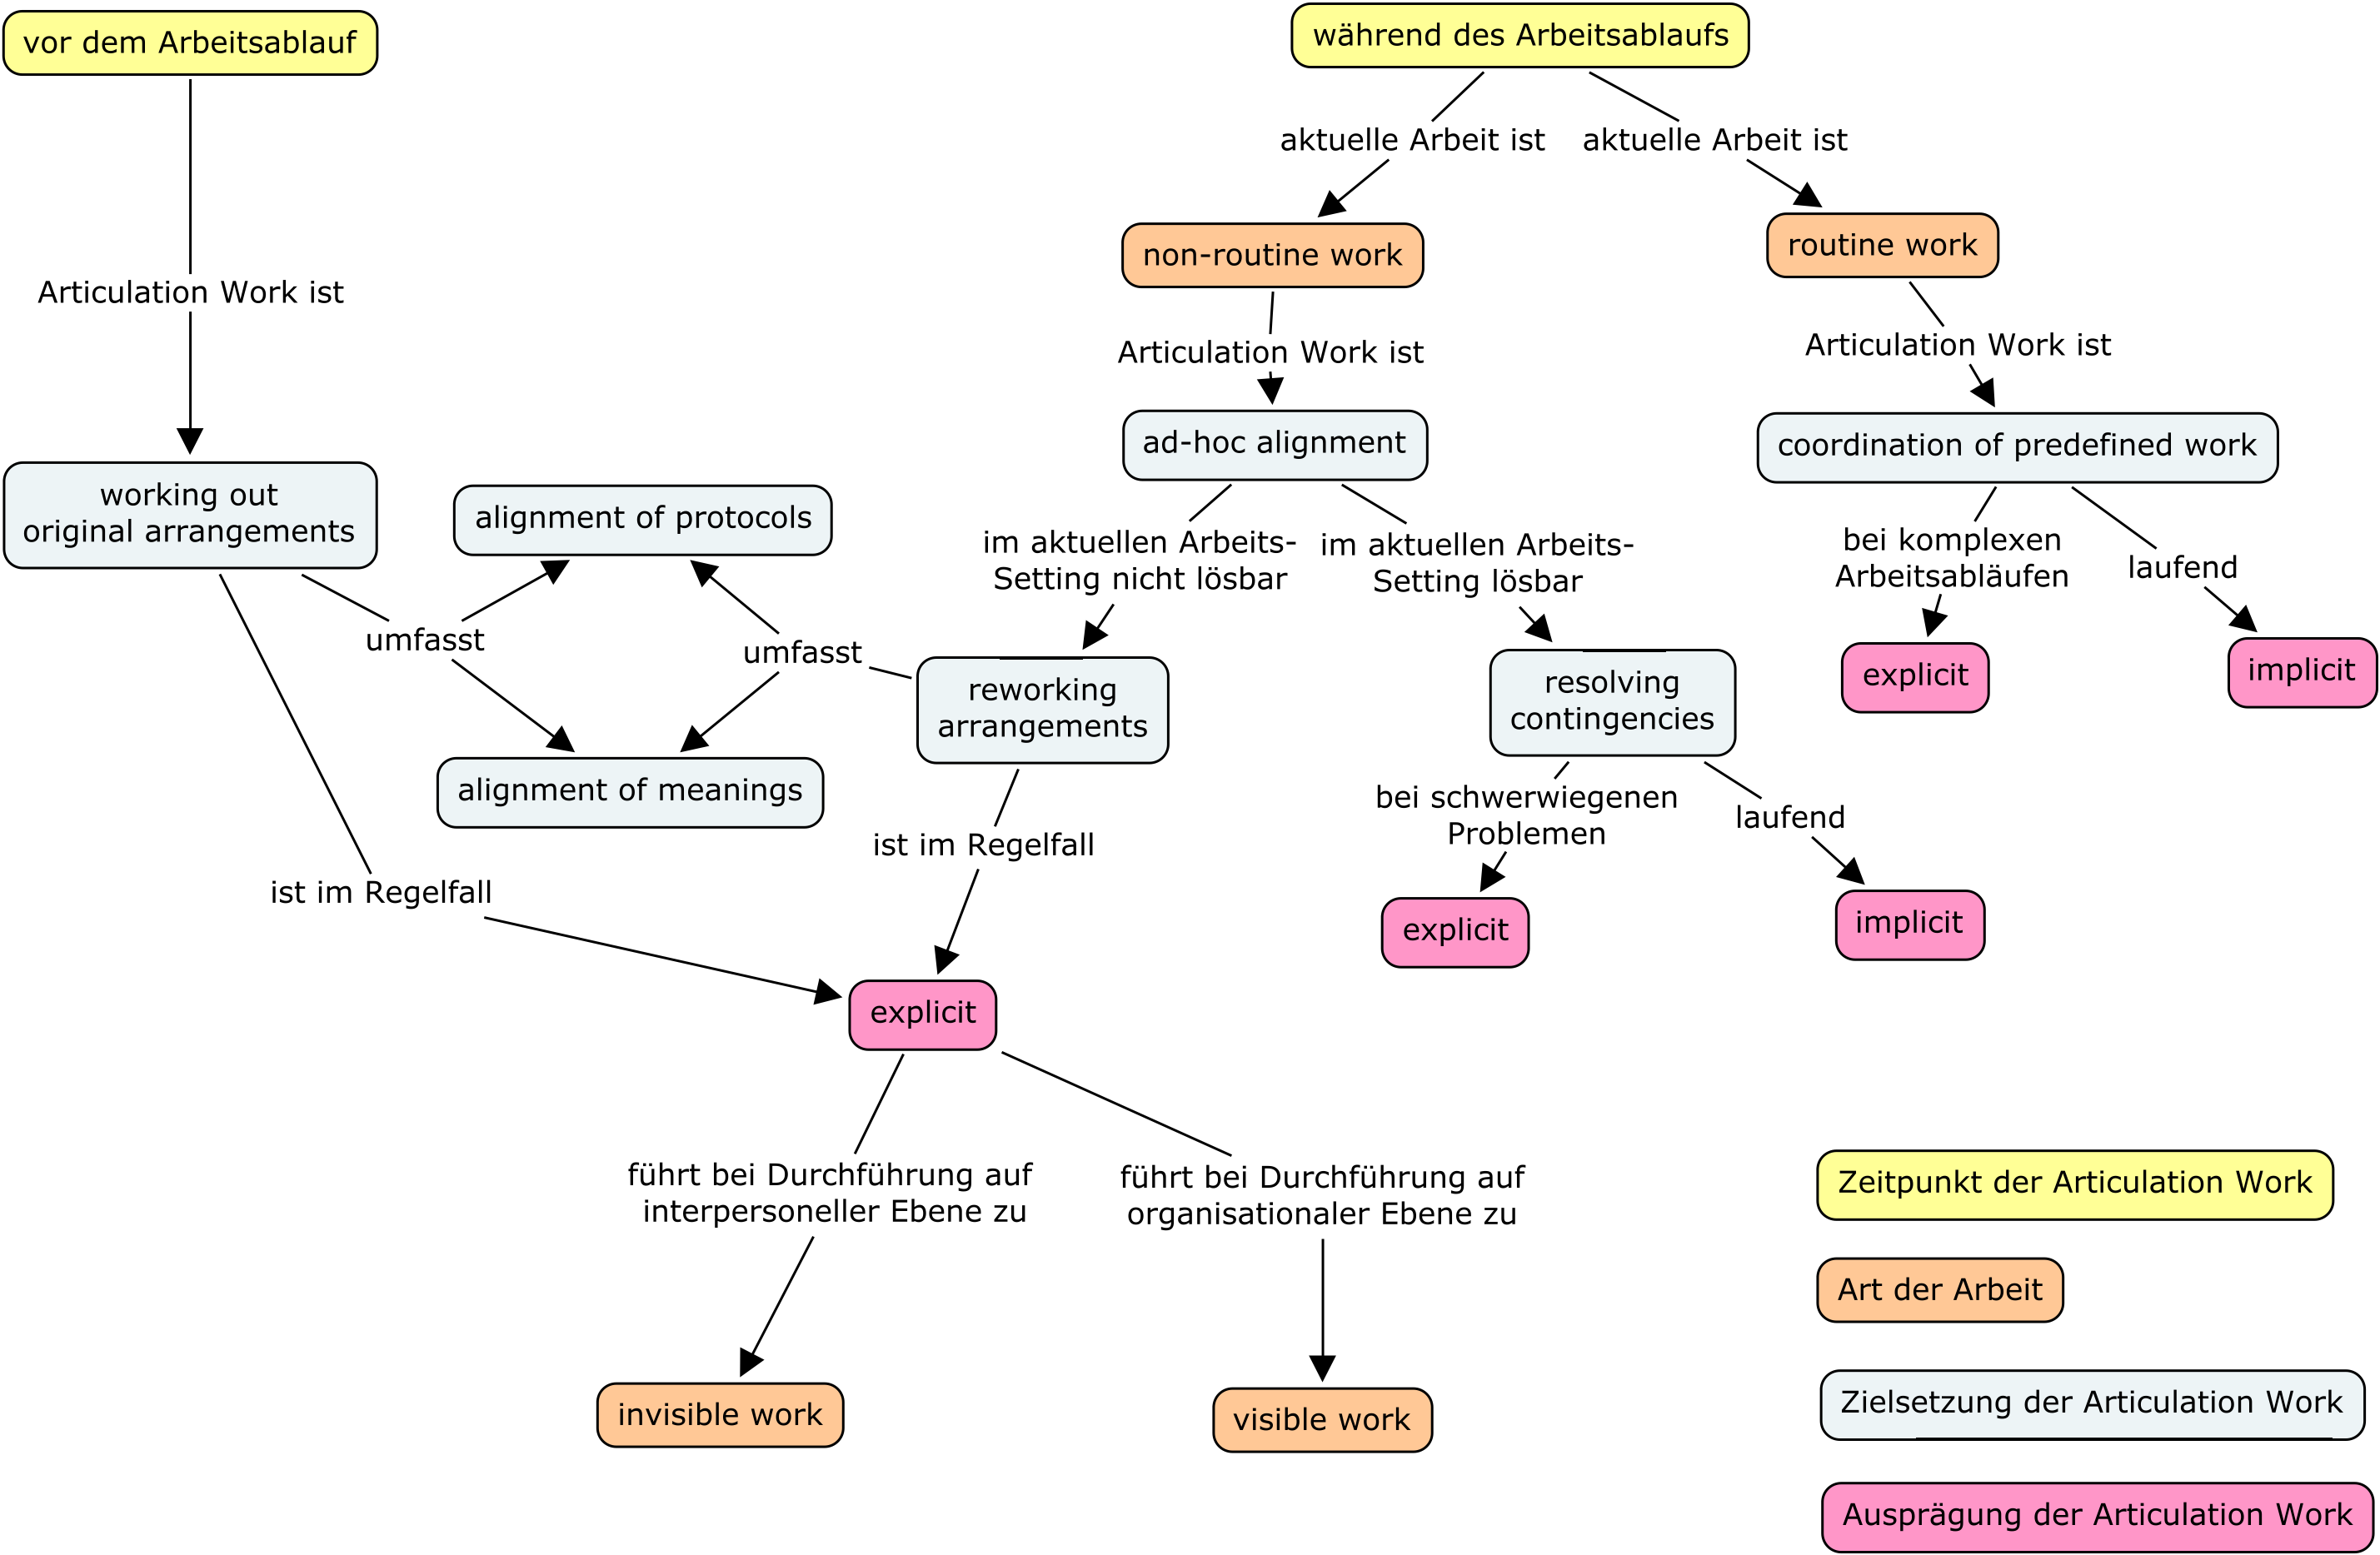
\includegraphics[width=\textwidth]{img/ArticulationWork/aw_conceptual_structure.png}
	\caption{Articulation Work im Durchführungskontext}
	\label{fig:img_ArticulationWork_aw_conceptual_structure}
\end{figure}

Die erste Unterscheidung, die am oberen Rand der Grafik dargestellt ist, betrifft den Zeitpunkt der Durchführung von „Articulation Work“. Während von den meisten Autoren lediglich jene Phasen eines Arbeitsprozesses zu „Articulation Work“ gezählt werden, die während der Durchführung der „Production Work“ auftreten, bezeichnen \citet{Corbin93} selbst auch den Vorlauf eines Arbeitsprozesses (also die Konzeptions- und Planungsphase) als „Articulation Work“ (auch die ursprüngliche Definition von Stauss schließt diese Phase nicht aus). Nach \citet{Corbin93} ist „Articulation Work“ in dieser Phase immer explizit (entsprechend dem in dieser Arbeit angegebenen Schema). Obwohl grundsätzlich nichts gegen eine implizite Durchführung dieser Phase spräche (bei „einfachen“ Arbeitsaufgaben, die von (etablierten Gruppen von) Individuen übernommen werden), wird diese Variante von den Autoren nicht erwähnt und deshalb in der Abbildung nicht dargestellt. Je nach Kontext, in dem die „Articulation Work“ durchgeführt wird (organisational, d.h. in offiziellem Rahmen oder informell ausschließlich in der lokalen Arbeitsumgebung) führt sie zu „visible“ oder „invisible work“.

„Articulation Work“, die im Zuge des Arbeitsablaufs ausgeführt wird, kann zwei Zwecken dienen. Einerseits kann sie im Falle etablierter Arbeitsabläufe („routine“) der Koordination der ohnehin definierten Abläufe dienen (die nicht notwendigerweise „visible“ sein müssen). Dies wird im Regelfall implizit ablaufen, lediglich bei komplexen Arbeitsabläufen oder etwa in verteilt organisierten Arbeitsumgebungen (vgl. \citep{Carstensen99}) wird eine explizite Beschäftigung mit der Koordination notwendig sein. Andererseits kann „Articulation Work“ auch in Situationen („ad-hoc“) zur Anwendung kommen, in denen keine etablierten Arbeitsabläufe existieren oder diese aufgrund von Veränderung in der Arbeitsumgebung nicht adäquat sind. Dieser Fall beschreibt „Articulation Work“ im engeren Sinne, die der Wiederherstellung der Arbeitsfähigkeit in Situationen dient, in denen die Ausführung von „Production Work“ (aus welchen Gründen auch immer) nicht mehr möglich ist.

Bei der „ad-hoc“-Anwendung von „Articulation Work“ sind unterschiedliche Eskalationsstufen zu unterscheiden. In vielen Situationen, die von einzelnen beteiligten Individuen als „problematisch“ oder „non-routine“ wahrgenommen werden, ist die Auflösung dieser Bedenken durch einfache implizite „Articulation Work“, also ohne bewusste Beschäftigung im Rahmen der üblichen sozialen Interaktion möglich. Wird die aktuelle Arbeit als so „problematisch“ wahrgenommen, dass sie nicht durchgeführt bzw. aufrecht erhalten werden kann, muss eine explizite (d.h. bewusste) Beschäftigung mit der Situation erfolgen, um die „Production Work“ wieder in einen operativen Zustand zu versetzen oder verbleibende Unklarheiten implizit beseitigen zu können. 

Es können jedoch Situation auftreten, in denen die aktuelle Arbeitspraxis nicht mehr soweit angepasst werden kann, dass die „Production Work“ wieder aufgenommen werden kann. Dies ist vor allem in Situationen der Fall, in denen es zu massiven Veränderungen des Arbeitskontexts gekommen ist (etwa durch veränderte Vorschriften, neue Werkzeuge oder Personaländerungen). In diesen Fällen muss die Arbeitspraxis selbst hinterfragt werden, was nach \citep{Corbin93} im Wesentlichen einer Neuplanung unter Berücksichtigung der bislang gemachten Erfahrungen entspricht. Diese Überarbeitung ist immer explizit und kann je nach Durchführungskontext wiederum zu „visible“ oder „invisible work“ führen. Sie umfasst je nach Art des aufgetretenen Problems „alignment of meaning“ (also die Entwicklung einer gemeinsamen Sicht aller beteiligten Individuen auf die Arbeitsdomäne) und / oder „alignment of procedures“ (also die Abstimmung der Modalitäten der Zusammenarbeit).

An dieser Stelle ist es wichtig, nochmals darauf hinzuweisen, dass die getroffenen Unterscheidungen keine strikte, präskriptive Kategorisierung von „Articulation Work“ darstellen. Wie auch von \citet{Schmidt00} angemerkt\footnote{\emph{„As already indicated, the general modalities of articulation work which we for the sake of clarity discussed separately — ad hoc alignment and improvisation on the basis of mutual awareness versus action constrained by coordinative artifacts and protocols — are not ‘natural kinds’ in the Aristotelian sense: they do not exist as distinct domains of action, they are analytical distinctions.“}\citep[][S. 7]{Schmidt00}}, sind die Grenzen zwischen den unterschiedlichen Ausprägungen von „Articulation Work“ fließend. Auch die Kontexte, die zur Durchführung einer bestimmten Ausprägung führen, sind dynamisch und können sich während der Durchführung der „Articulation Work“ selbst ändern. Für diese Arbeit bedeutet dies, das sich die Unterstützung von „Articulation Work“ nicht auf eine bestimmte Ausprägung beschränken darf -- vielmehr muss ein Weg gefunden werden, unterschiedliche Anforderungen an die gegenseitige Abstimmung in unterschiedlichen Kontexten zu realisieren.

In der Darstellung nicht enthalten sind die Unterscheidungen, die nach \citep{Fjuk97} auf die „Activity Theory“ zurückzuführen sind. Es sind dies die Unterscheidung nach Kooperations-Art der Arbeit („individuell“ vs. „lose kooperativ“ vs. „eng kooperativ“) und dem Abstraktionsgrad der „Articulation Work“ (abstrakt zwischen „activity“ und „action“ vs. konkret zwischen „action“ und „operation“). Hintergrund der Entscheidung, diese Unterscheidungen in der Abbildung zu vernachlässigen, ist deren fehlende Wirkung auf die Ausprägung der durchgeführten „Articulation Work“ (implizit oder explizit). In allen Kooperations-Arten ist die Durchführung von sowohl impliziter als auch expliziter „Articulation Work“ auf beiden Abstraktionsstufen denkbar. Es ändert sich lediglich die konkrete Ausgestaltung der „Articulation Work“ bzw. die Notwendigkeit einer eventuellen Unterstützung.

Außerdem fehlt in der Darstellung die Unterscheidung anhand der Reichweite von „Articulation Work“ nach \citep{Faergemann05}. Diese hat durchaus Einfluss auf die Ausprägung der durchgeführten „Articulation Work“, steht aber vollständig orthogonal zu den abgebildeten Unterscheidungen. Die Komplexität der Darstellung wäre deshalb durch die Integration dieser Unterscheidung auf ein Maß angestiegen, das eine sinnvolle Interpretation der Grafik nicht mehr zugelassen hätte. Die Reichweite ist deshalb implizit in der Unterscheidung nach „routine“ und „non-routine work“ codiert, da domänenübergreifende Arbeitssituationen tendenziell eher „non-routine“ bzw. „problematic“ sind und dadurch eher zu expliziterer „external Articulation Work“ führen.

Auf Basis dieser dargestellten Struktur werden die im folgenden Abschnitt beschriebenen Arbeitsaspekte in unterschiedlichen Ausprägungen von „Articulation Work“ abgestimmt bzw. koordiniert. Jede dieser Ausprägungen muss in den unterschiedlichen Kontexten, in denen sie auftreten können, verschieden stark und mit unterschiedlichen Mitteln unterstützt werden. Abschnitt \ref{sec:unterstützung_von_articulation_work} widmet sich auf Basis einer Literaturstudie dem State-of-the-Art der Möglichkeiten dieser Unterstützung aus organisationer, methodischer und technischer Sicht.

% subsection aw_zusammenfassung (end)
% section arten_von_articulation_work (end)

\section{Abzustimmende Arbeitsaspekte} % (fold) 
\label{sec:abzustimmende_arbeitsaspekte}

Bei der Durchführung von „Articulation Work“ ist das Ziel etwaige im Rahmen eines Arbeitsablaufs aufgetreten Unklarheiten oder Probleme aufzulösen. Diese Probleme und Unklarheiten können unterschiedliche Aspekte der Arbeit (etwa die durchzuführenden Schritte, die beteiligten Personen und Verantwortlichkeiten oder die zu verwendenden Ressourcen) betreffen. Um „Articulation Work“ umfassend zu beschreiben und eine fundierte Unterstützung gewährleisten zu können, ist eine nähere Beschäftigung mit diesen potentiell abzustimmenden Arbeitsaspekten notwendig.

Abbildung \ref{fig:img_ArticulationWork_schmidt96-articulation-categories} zeigt eine Übersicht über Aspekte, die im Rahmen von „Articulation Work“ Gegenstand der Abstimmung zwischen den beteiligten Individuen sein können (entnommen aus \citep{Schmidt96}). In Abbildung \ref{fig:img_ArticulationWork_divitini00_caw} sind diese Aspekte nochmals hinsichtlich der Zusammenhänge zwischen ihnen diagrammatisch dargestellt.

\begin{figure}[htbp]
	\centering
	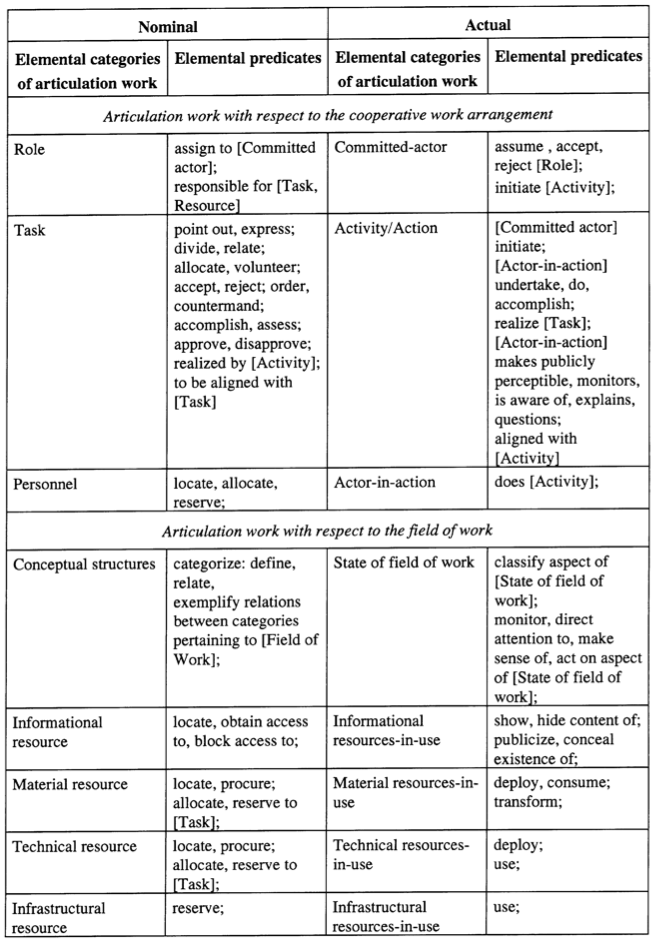
\includegraphics[height=6in]{img/ArticulationWork/schmidt96-articulation-categories.png}
	\caption[Abzustimmende Arbeitsaspekte]{Abzustimmende Arbeitsaspekte (entnommen aus \citep{Schmidt96})}
	\label{fig:img_ArticulationWork_schmidt96-articulation-categories}
\end{figure}


Obwohl diese Übersicht aus Beobachtungen induktiv abgeleitet ist und keinen Anspruch auf Vollständigkeit erhebt, zeigt sie doch eine Anzahl von konkreten Ausprägungen der von Strauss angeführten Dimensionen von Arbeit, die im Rahmen von „Articulation Work“ abzustimmen sind („Wer?“, „Was?“, „Wann/Wo?“ und „Wie?“). Die Autoren klären also, welche Aspekte von Arbeit konkret von der Abstimmung betroffen sein können. Mit der Unterscheidung zwischen den nominalen Aspekten von Arbeit und der konkreten Manifestation eines Arbeitsablaufs im organisationalen Kontext stellen die Autoren einen in dieser Form bislang nicht explizit angesprochenen Unterschied bei der Durchführung von „Articulation Work“ dar.

Konzeptuell unterscheiden die Autoren auch zwischen Arbeitsaspekten, die den Arbeitsablauf an sich betreffen (\emph{„cooperative work arrangement“}) und Aspekten, die den Durchführungsrahmen der Arbeit, also deren Umfeld oder organisationalen Kontext beschreibt (\emph{„field of work“}). Die Berücksichtigung beider Aspekte wird bereits bei \citet{Strauss88} als ein wesentliches Merkmal von „Articulation Work“ identifiziert, bei \citet{Schmidt96} aber erstmals in dieser expliziten Form dargestellt und abgegrenzt.

Konkret nimmt also die Frage nach dem „Womit?“ -- also den Arbeitsmitteln, den Ressourcen bzw. dem Arbeitsumfeld an sich --  sowohl auf konzeptueller als auch auf konkreter Ebene eine großen Stellenwert ein. Die Behandlung dieses Aspektes dient vor allem der Bildung einer gemeinsamen Sichtweise auf den Arbeitskontext, in dem der betreffende Arbeitsablauf abgehandelt wird.

\begin{figure}[htbp]
	\centering
		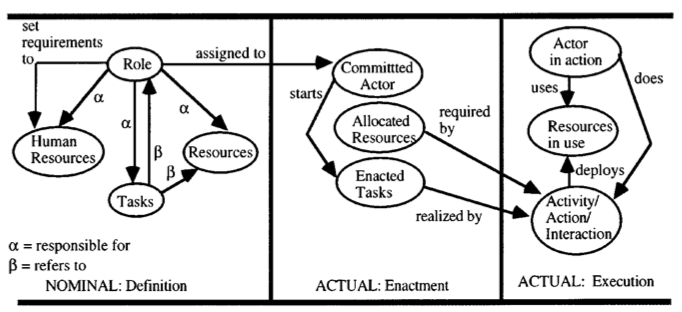
\includegraphics[width=10cm]{img/ArticulationWork/divitini00_caw.png}
	\caption[Zusammenhänge zwischen Arbeitsaspekten]{Zusammenhänge zwischen Arbeitsaspekten (entnommen aus \citep{Divitini00})}
	\label{fig:img_ArticulationWork_divitini00_caw}
\end{figure}

Von Interesse sind auch die den einzelnen Aspekten zugeordneten Prädikate, die eine Aussage über die konkret durchzuführenden Aktivitäten zulassen. Diese Aktivitäten sind sowohl dem Bereich der „Production Work“ (z.B. „do“, „use“) als auch der „Articulation Work“ zuzuordnen (z.B. „assign to“, „allocate“). Zum Teil sind auch Beziehungen zwischen den Aspekten angeführt, die eine notwendige Abstimmung über die Grenzen der einzelnen Aspekte hinweg anzeigen (z.B. „Task realized by Activity“ oder „Role responsible for Task“).

Für diese Arbeit ist die Beschreibung der abzustimmenden Aspekte von Interesse, als dass an diesen die Effektivität der Durchführung von „Articulation Work“ beobachtet werden kann. Diese Effektivität ist dann gegeben, wenn eine gemeinsame Sichtweise auf die abzustimmenden Gegenstände, konkret also die relevanten Aspekte des Arbeitsablaufs selbst sowie jene aus dessen Umfeld, entwickelt wurde.

% section abzustimmende_arbeitsaspekte (end)

\section{Unterstützung von Articulation Work} % (fold)
\label{sec:unterstützung_von_articulation_work}

Nach den ersten Arbeiten von Strauss zum Thema „Articulation Work“ wurde das Konzept bald als Erklärungsmodell für die Vorgänge aufgenommen, die im Zuge kooperativer Arbeit ablaufen. Bereits \citeyear{Gerson86} verweisen \citeauthor{Gerson86} auf die Notwendigkeit einer expliziten Unterstützung von „Articulation Work“\footnote{\emph{„Methods for analyzing 
due process means, in this perspective, explicit procedures for evaluating and reconciling incompatibilities among different bodies of tacit local knowledge.“}\citep[][S. 266]{Gerson86}}. Anhand der historischen Entwicklung von Mitte der 1980er-Jahre bis Ende des ersten Jahrzehntes des neuen Jahrtausends werden in den folgenden Abschnitten Maßnahmen zur Unterstützung beschrieben und in den jeweiligen Anwendungskontext gesetzt. Hierbei werden alle Arbeiten berücksichtigt, die sich direkt auf den von Strauss geprägten „Articulation Work“-Begriff beziehen. 

In der Literatursuche wurden dazu Datenbanken aus den Bereichen Informatik, Psychologie, Soziologie, den Wirtschaftswissenschaften sowie der Organisationslehre durchsucht (für eine detaillierte Auflistung siehe Abschnitt \ref{sec:literaturquellen}). Nach der initialen Suche wurde jeweils auch die in den gefundenen Arbeiten referenzierte Sekundärliteratur aufgearbeitet. Des weiteren wurden mit Hilfe von rückwärts verlinkenden Datenbanken (wo vorhanden) Publikationen erfasst, die die bislang gefundenen Arbeiten referenzieren und diese hinsichtlich ihrer Relevanz überprüft. Insgesamt ergab sich so eine Sammlung von 70 Publikationen (inklusive der grundlegenden Arbeiten, die bereits oben beschrieben wurden). Von diesen 70 Publikationen wurden 13 Arbeiten im Kontext dieses Abschnitts einer näheren Betrachtung unterzogen, da sie Aussagen zur Unterstützung von „Articulation Work“ treffen. Die übrigen Publikationen geben hierzu keine Aussage ab oder sind im Kontext größerer Forschungsvorhaben entstanden, die bereits durch eine repräsentative Arbeit in der detaillierten Betrachtung enthalten sind. 

Sämtliche Arbeiten sind in Anhang \ref{cha:literatur_zum_themengebiet_articulation_work} hinsichtlich ihres Inhalts beschrieben und ihrer Relevanz für die Unterstützung von „Articulation Work“ beurteilt. In Anhang \ref{cha:literatur_zum_themengebiet_articulation_work} ist außerdem eine Übersichtsgrafik zu finden, die das gesamte Feld an Publikationen zum Thema „Articulation Work“ visualisiert und die Zusammenhänge zwischen den einzelnen Arbeiten und Forschungsvorhaben aufzeigt.

\subsection{Vorgehen zur detaillierten Betrachtung} % (fold)
\label{sub:vorgehen_zur_detaillierten_betrachtung}

Zur strukturierten Betrachtung der Unterstützung von „Articulation Work“ wird ein einheitlicher Raster angewandt, anhand dessen die aus unterschiedlichen Forschungsgebieten stammenden und in unterschiedlichen Anwendungsdomänen angewandten Arbeiten einander gegenüber gestellt werden können. Neben den eigentlichen Unterstützungsmaßnahmen ist zur Bewertung derselben auch Kontextinformation notwendig, die die unterschiedlichen Ansätze offenlegt. Folgende Merkmale bzw. Inhalte einer Arbeit werden dazu betrachtet:

\begin{description}
	\item[Kontext] Forschungsgebiet aus dem das Konstrukt „Articulation Work“ betrachtet wird bzw. in dessen Kontext es zur Anwendung gebracht wird und / oder abstraktes oder konkretes Problemfeld, in dem „Articulation Work“ als Analysedimension oder zur Ableitung von Maßnahmen angewandt wird.
	\item[Unterstützung] Konkrete oder abstrakte Maßnahmen oder Werkzeuge, die zur Unterstützung von „Articulation Work“ vorgeschlagen und/oder umgesetzt werden. Ggf. unterschieden in
	\begin{itemize}
		\item organisationale Unterstützung
		\item methodische Unterstützung
		\item technische Unterstützung
	\end{itemize}
	\item[Auswirkungen] Tatsächliche oder vermutete Auswirkungen der Unterstützung auf die durchgeführte „Articulation Work“.
	\item[Bewertung] Zusammenfassung des Beitrags der Arbeit zur Unterstützung von „Articulation Work“ hinsichtlich der unterstützten Ausprägungen inklusive einer Beurteilung der möglichen Generalisierbarkeit der vorgeschlagenen Maßnahmen bzw. vorgestellten Werkzeuge.
\end{description}

Die als relevant betrachteten Publikationen sind methodisch unterschiedlich ausgerichtet. Ein großer Anteil beschreibt rein empirisch-deskriptiv ein beobachtetes Phänomen und zieht Schlüsse hinsichtlich möglicher bzw. notwendiger Ausprägungen von „Articulation Work“ in bestimmten Anwendungsdomänen. Ein anderer Teil fokussiert auf die organisationale und/oder technische Unterstützung von „Articulation Work“, zum Teil ohne auf eigene empirische Ergebnisse aufzubauen oder diese zu erheben. Aus diesem Grund kann das oben angegebene Raster nicht immer vollständig befüllt werden. Wo hinsichtlich einer bestimmten Dimension keine Information vorhanden ist, wird explizit im Text darauf hingewiesen. Wo mehrere Publikation eines Autors oder einer Gruppe zum gleichen Forschungsgegenstand existieren, wurden die als am umfassendsten erscheinenden Arbeiten (i.A. jene, die das jeweilige Forschungsvorhaben abschließend beschreiben) herausgegriffen und exemplarisch detailliert ausgearbeitet. Alle übrigen Arbeiten des Forschungsgegenstandes \ref{cha:literatur_zum_themengebiet_articulation_work} sind in entsprechend der jeweils hier beschriebenen Publikation zugeordnet.

% subsection vorgehen_zur_detaillierten_betrachtung (end)

\subsection{Modeling Articulation Work in Software Engineering Processes} % (fold)
\label{sub:modeling_articulation_work_in_software_engineering_processes}

Die erste Publikation, die sich mit der organisationalen Unterstützung von „Articulation Work“ in Form der expliziten Berücksichtigung von „Articulation Work“ in formalisierten Ablaufmodellen beschäftigt, ist die Arbeit von \citet{Mi91}.

\subsubsection{Kontext}

\citet{Mi91} betrachten „Articulation Work“ im Kontext der Softwareentwicklung und argumentieren für deren explizite Berücksichtigung in Software Engineering Prozessen. In einer Literaturstudie zeigen sie, dass (die zum Zeitpunkt der Erstellung) verfügbaren Software-Engineering-Prozess-Modellierungs-Techniken die Einbindung von „Articulation Work“ in die Vorgehensmodelle nicht ermöglich\footnote{\emph{„After we compare these findings with the process modeling techniques, it becomes apparent that current software process modeling techniques do not directly address articulation work.“}\citep[][S. 192]{Mi91}}. Die Autoren selbst haben ihren Hintergrund ebenfalls in der Domäne des Software Engineering und wählen ihren Zugang zu Thematik dementsprechend, indem sie eine formale Abbildung des „Articulation Work“-Prozesses und eine Unterstützung durch regelbasierte Heuristiken zur Lösungsfindung vorschlagen.

\subsubsection{Unterstützung}

Die Autoren formalisieren im ersten Schritt den Ablauf von „Articulation Work“ im Kontext von Softwareengineering (siehe Abbildung \ref{fig:img_ArticulationWork_mi91-awprocess}). Die einzelnen Schritte leiten sie aus drei empirischen Studien ab, die sowohl hinsichtlich ihres Inhalts als auch ihrer Durchführung nicht näher beschrieben werden.

\begin{figure}[htbp]
	\centering
		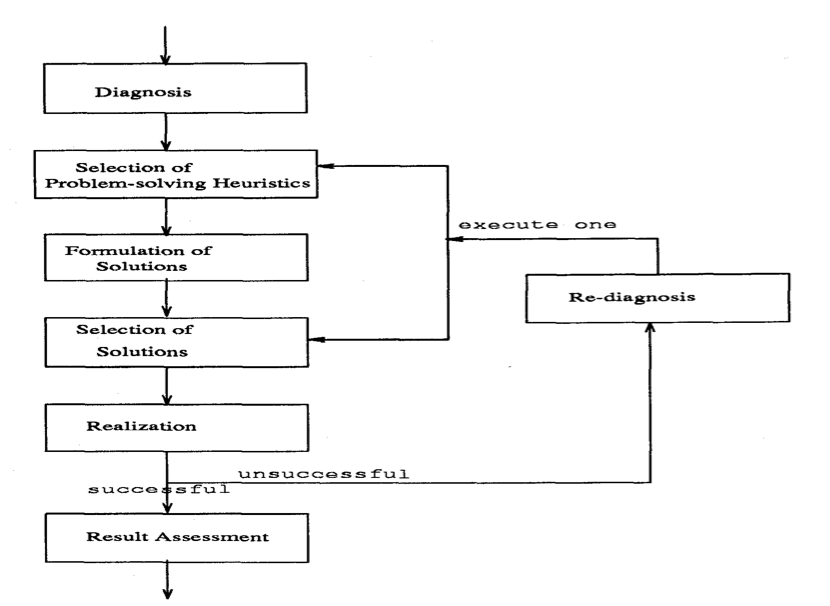
\includegraphics[height=3in]{img/ArticulationWork/mi91-awprocess.png}
	\caption[Artikulations-Prozess]{Artikulations-Prozess (entnommen aus \citep{Mi91})}
	\label{fig:img_ArticulationWork_mi91-awprocess}
\end{figure}

Die Autoren beziehen sich also offensichtlich auf explizite „Articulation Work“, die „ad-hoc“ -- beim Auftreten eines Problems im Software Engineering Prozess -- ausgelöst wird.

Zur Durchführung dieses Prozesses schlagen die Autoren einen Satz von regelbasierten Heuristiken vor, aus denen die betroffenen Individuen (hier: „agents“) auswählen können. Diese Heuristiken beschreiben mögliche Tätigkeiten im Zuge der „Articulation Work“ (ausdefiniert durch \gls{ECA}-Regelsätze). Dabei geben die Autoren Heuristiken zur Problemlösung („problem-solving heuristics“, die der direkt Behebung der aufgetretenen Probleme dienen) und Heuristiken zur Auswahl geeigneter Lösungen („selection heuristics“) an.

\subsubsection{Auswirkungen}

Das vorgeschlagene System wurde auf konzeptueller Ebene entwickelt und nicht praktisch umgesetzt. Insofern existieren keinerlei reale Erfahrungen mit dem Ansatz. Anhand eines hypothetischen Beispiels demonstrieren die Autoren jedoch die Anwendung des Modells und der Heuristiken.

Der Vorteil liegt im Wesentlichen darin, dass der „Articulation Work“-Prozess durch seine Formalisierung bekannt ist („visible“ in Sinne der Ausführungen in Abschnitt \ref{sub:arten_hampson}) und dementsprechend auch offiziell auftreten „darf“. Durch den vorgegebenen Satz an Heuristiken sind außerdem die Alternativen zur Problembehandlung und deren Durchführung bekannt. Die Autoren geben diese Heuristiken für den Bereich des Software-Engineering an, betonen aber deren exemplarischen Charakter -- die Heuristiken und vor allem deren konkrete Umsetzung (durch die Spezifikation von \gls{ECA}-Regeln) müssen an die jeweilige Arbeits-Domäne angepasst werden. 

\subsubsection{Bewertung}

Das vorgeschlagene Prozess-Modell von „Articulation Work“ bildet den Ablauf auf so abstrakter Ebene ab, dass es für „ad-hoc explicit Articulation Work“ zur Lösung unmittelbar auftretender Probleme allgemein (d.h. unabhängig von der Anwendungsdomäne) anwendbar erscheint und auch in mit den von \cite{Corbin93} genannten Schritten bei der Durchführung expliziter „Articulation Work“ in Einklang gebracht werden kann.

Die Angabe von (exemplarischen) Heuristiken zur Durchführung des Artikulations-Prozesses erscheint insofern sinnvoll, als dass diese domänen- und organisations-spezifische Lösungsstrategien auch für unerfahrene Teilnehmer zugänglich machen können.

In Bezug auf die Generalisierbarkeit des Ansatzes problematisch zu sehen ist jedoch die Verwendung von \gls{ECA}-Regeln zur Spezifikation der Durchführung der einzelnen Heuristiken. Die Angabe derartiger Regeln erscheint nicht in allen Anwendungsbereichen in einem sinnvollen Detaillierungsgrad möglich zu sein. Vor allem soziale Prozesse in kooperativen Umgebungen, auf die die Autoren der ursprünglichen Literatur zum Thema „Articulation Work“ stark Bezug nehmen, können in diesen Regeln nicht sinnvoll (im Sinne einer Durchführungsvorschrift) abgebildet werden.
\\[1em]
\begin{tabular}{| p{3cm} | p{10cm} |}
  \hline
  Kontext & Unterstützung von Software Engineering \\ \hline
  Art von AW & ad-hoc explizit \\ \hline
  Unterstützung & \emph{organisational} durch Formalisierung und a-priori-Spezifikation des Articulation-Prozesses („Was?“) und dessen Ausgestaltung („Wie?“) \\ \hline
  Auswirkungen & Definiertes Vorgehen, wie „Articulation Work“ durchgeführt werden muss \\ \hline
\end{tabular}

% subsection subsection_name (end)

\subsection{Taking CSCW seriously: Supporting Articulation Work}

\citet{Schmidt92} begründen mit dieser Arbeit eine Entwicklungsrichtung der \gls{CSCW}, die neben der Unterstützung der eigentlichen produktiven Arbeit auch auf die Unterstützung von „Articulation Work“ fokussiert. Sie beschreiben damit erstmals Anforderungen an die und Möglichkeiten der technische Unterstützung von „Articulation Work“.

\subsubsection{Kontext}

\citet{Schmidt92} widmen sich in ihren Ausführungen der kooperativen Arbeit und der Unterstützung derselben durch Computersysteme. Sie argumentieren, dass zum Zeitpunkt der Erstellung der Arbeit \gls{CSCW} auf einer sehr formalisierten, strukturierten Sichtweise von kooperativer Arbeit aufbaut (z.B. im Sinne einer präskriptiven Workflow-Unterstützung) und Aspekte wie individuelle Arbeitsweise und Kommunikation unter den Beteiligten vernachlässigt. Dieser Sichtweise setzen sie einen Ansatz entgegen, der auch die Unterstützung von „Articulation Work“ berücksichtigt und damit den handelnden Individuen selbst die Kontrolle über die Interaktion gibt\footnote{\emph{„Thus, by entering into cooperative work relations, the participants must engage in activities that are, in a sense, extraneous to the activities that contribute directly to fashioning the product or service and meeting requirements.“}\citep[][S. 8]{Schmidt92}}.

Die Autoren selbst arbeiten vor ihrem Hintergrund aus der Informatik, der Soziologie und den Arbeitswissenschaften. Sie stellen die Technologie nicht ins Zentrum ihrer Überlegungen, sondern betonen deren unterstützende Funktion für  Individuen, die in Organisationen arbeiten. Die Untersuchungsdomäne ist dabei explizit nicht eingeschränkt, kooperative Arbeit wird in allen ihren Ausprägungen und in beliebigen Kontexten betrachtet\footnote{\emph{„In sum, we certainly want CSCW to address the aspects of computer support for cooperative work wherever they occur.“}\citep[][S. 11]{Schmidt92}}.

\subsubsection{Unterstützung}

Bei ihren Ausführungen zur unterstützenden Wirkung von \gls{CSCW} bei „Articulation Work“ konzentrieren sich die Autoren auf zwei Aspekte von \gls{CSCW} und zeigen, wie diese ausgestaltet sein müssen, um „Articulation Work“ zuzulassen bzw. zu unterstützen. 

Der erste Aspekt, auf den eingegangen wird, ist die Unterstützung von Workflows durch Computersysteme. Um hier „Articulation Work“ zu berücksichtigen, ist die Unterstützung der Selbst-Organisation der kooperierenden Personen ein zentraler Punkt\footnote{\emph{„Computer support of cooperative work should aim at supporting self-organization of cooperative ensembles as opposed to disrupting cooperative work by computerizing formal procedures.“}\citep[][S. 17]{Schmidt92}}. In diesem Sinne argumentieren die Autoren gegen einen fixen, unveränderlich vorgegebenen Workflow mit a-priori definierten Zuständigkeiten, sondern schlagen die Ermöglichung bzw. Unterstützung von Aushandlungsprozessen vor, in denen der Arbeitsablauf entsprechend dem aktuellen Arbeitskontext angepasst und kooperativ abgearbeitet werden kann. Anhand der angeführten Beispiele wird deutlich, dass dabei eher von „Articulation Work“ zur Koordinierung etablierter Arbeitsprozesse ausgegangen wird, die vorgeschlagene Unterstützungsfunktionalität ist jedoch auch für „ad-hoc Articulation Work“ sinnvoll anzuwenden (in Klammer jeweils die Zuordnung zur Art von „Articulation Work“):
\begin{itemize}
	\item Offenlegung des der Workflowunterstützung zugrunde liegenden Modells und Unterstützung der Interpretation und Reflexion desselben („ad-hoc implicit and explicit Articulation Work“)
	\item Unterstützung der Anpassung des Modells an den aktuellen Arbeitskontext („explicit resolving contingencies“)
	\item Ermöglichung der flexiblen Anwendung bzw. dynamischen Veränderung des Modells während der Ausführung des Arbeitsablaufs („implicit and explicit coordination of predefined work“)
	\item Unterstützung zur Veränderung bzw. Neuerstellung von Modellen, um die Arbeit an veränderte organisationale Rahmenbedingungen anzupassen („reworking arrangements“)
	\item Dokumentation und Kommunikation aller Veränderungen des Modells oder Abweichungen während der Ausführung (in allen Fällen)
	\item Unterstützung der Aushandlung eines gemeinsamen Verständnisses des Modells („ad-hoc explicit Articulation Work“)
\end{itemize}

Der zweite Aspekt, auf den näher eingegangen wird, ist jener der Kooperation mittels geteilter Informationsräume, also Ablagesysteme für Informationen, auf die mehrere Personen Zugriff haben. Als zentral wird hier die Unterstützung der Entwicklung einer einheitlichen Interpretation der verfügbaren Information gesehen\footnote{\emph{„At the level of the objects themselves, shareability may not be a problem, but in terms of their interpretation, the actors must attempt to jointly construct a common information space which goes beyond their individual personal information spaces.“}\citep[][S. 21]{Schmidt92}}. Die Autoren führen hier drei Funktionen an, die ein \gls{CSCW}-System unterstützen muss:
\begin{itemize}
	\item Unterstützung der Identifikation des Erstellers die Information
	\item Offenlegung der Kontexts der Information (im Sinne einer Relation zur Ursprungs- bzw. Anwendungsdomäne)
	\item Kontrolle über den Zugriff auf Information durch den Ersteller
\end{itemize}
Die genannten Aspekte zielen allesamt nicht auf die Unterstützung direkter Interaktion ab, sondern ermöglichen durch die Erfassung von Metadaten im Wesentlichen eine Beurteilung von geteilt verfügbarer Information durch Individuen, während diese damit arbeiten. Die „Articulation Work“, die hier unterstützt wird, ist durch die semi-automatisierte Erfassbarkeit bzw. die automatisierte Anzeige zumeist implizit. 

\subsubsection{Auswirkungen}

Aufgrund der konzeptuellen Natur der Arbeit stehen keine Angaben zu etwaigen Auswirkungen der Maßnahmen zur Verfügung.

\subsubsection{Bewertung}

\citet{Schmidt92} sind die ersten, die sich mit der technischen Unterstützung von „Articulation Work“ in beliebigen Anwendungsdomänen und in all ihren Ausprägungen beschäftigen. Sie geben dabei Anforderungen („Was?“) an diese technische Unterstützung an, gehen jedoch nicht auf deren Umsetzung („Wie?“) ein.

Auf Anforderungsebene wird jedoch umfassend hinsichtlich unterschiedlicher Artikulations-Bedürfnisse argumentiert, so dass die Arbeit als Grundlage zur Konzeption einer konkreten technischen Unterstützung von „Articulation Work“ herangezogen werden kann.
\\[1em]
\begin{tabular}{| p{3cm} | p{10cm} |}
  \hline
  Kontext & Umsetzung von \gls{CSCW}-Systemen (Workflow-Support, Shared Information Spaces, Cooperative Tools)\\ \hline
  Art von AW & alle Arten und Ausprägungen von „Articulation Work“ (Workflow Planung und Unterstützung), implizit (Information Sharing)\\ \hline
  Unterstützung & \emph{technisch} durch Maßnahmen, die sowohl die selbstgesteuerte Anpassung von Arbeitsabläufen an den aktuellen Arbeitskontext als auch die Entwicklung eines gemeinsamen Verständnis über den Arbeitsablauf und die verwendeten Arbeitsartefakte ermöglicht \\ \hline
  Auswirkungen & --- \\ \hline
\end{tabular}

\subsection{Supporting articulation work using software configuration management systems}
\label{sub:supporting_articulation_work_using_software_configuration_management_systems}

\citet{Grinter96} führt in dieser Arbeit die Ideen von \citet{Bendifallah87} und \citet{Schmidt92} weiter und zeigt, wie die Softwareentwicklung als kooperativer Prozess durch computerbasierte Werkzeuge unterstützt werden kann.

\subsubsection{Kontext}

Die Autorin betrachtet die Rolle von „Articulation Work“ im Kontext der Softwareentwicklung und zeigt anhand zweier qualitativer empirischer Studien die Auswirkungen eines computerbasierten Configuration Management Systems bei der kooperativen Erstellung von Software. 

\citeauthor{Grinter96} beschäftigt sich mit zwei Arten von Aufgaben, die im Rahmen eines Software-Entwicklungs-Prozesses im Rahmen von „Articulation Work“ zu bewältigen sind. Einerseits ist die tägliche Arbeit abzustimmen, so dass sichergestellt ist, dass die gerade erstellte Software korrekt funktioniert. Andererseits muss sichergestellt werden, dass auch das gesamte Produkt als Einheit funktioniert. Während die erstere Herausforderung durch das in den Fallstudien eingesetzte Configuration Management System unterstützt wurde (im Rahmen von „resolving contingencies“, die sowohl implizit als auch explizit war), waren im zweiten Fall organisationale Maßnahmen wie die Bildung von Koordinations-Kommitees (also „explicit coordination of predefined work“) notwendig. 

\subsubsection{Unterstützung}

In der Arbeit detailliert beschrieben sind die Eigenschaften und Auswirkungen des Configuration Management Systems, so dass hier nur dessen Unterstützungsleistung berücksichtigt werden kann. Konkret muss hier weiter auf jene Fälle von „resolving contingencies“ eingeschränkt werden, die von Problemen in Arbeitsabläufen ausgelöst werden, die auf konfliktionierende (Teil-)Ergebnisse der produktiven Arbeit zurückzuführen sind (hier: simultan editierter Source-Code, der nicht automatisiert zusammengeführt werden kann)

Während der Entwicklung von Software wird durch das Configuration Management System dargestellt, ob bzw. durch wen ein bestimmter Teil des Source Codes zur Zeit bearbeitet wird. So kann die simultane und potentiell zu Konflikten führende Bearbeitung durch andere Personen vermieden werden. Diese Information muss weder explizit ins System eingepflegt noch abgerufen werden und ist deshalb als Unterstützung von impliziter „Articulation Work“ zu klassifizieren.

Sind bereits Konflikte aufgetreten, unterstützt das System die Auflösung derselben durch eine adäquate Darstellung der betroffenen Teile des Source Codes, so dass den zusammenarbeitenden Individuen eine Grundlage zur Erörterung und Auflösung des Konflikts zur Verfügung steht. Diese Darstellung muss „geeignet“ sein -- welche Arten von Zusatzinformation und welche Form der Darstellung dies gewährleistet, ist domänenabhängig. Im konkreten Fall wird die zusätzliche Angabe einer Begründung für Änderungen in Source Code Teilen empfohlen, um bei der Auflösung der Konflikte fundiert argumentieren zu können.

\subsubsection{Auswirkungen}

Den Software Entwicklern wird die Freiheit gelassen, Konflikte durch sequentielle Bearbeitung zur vermeiden oder diese (z.B. aus Zeitdruck) bewusst in Kauf zu nehmen und deren Auflösung ggf. in einem separaten Schritt durchzuführen.

\subsubsection{Bewertung}

Die Arbeit von \citet{Grinter96} geht auf einen Spezialfall von „resolving contingencies“ ein und zeigt, welche Unterstützungsleistung ein Software-Werkzeug bei der Ausgestaltung eines Arbeitsprozesses leisten kann, in dem sich die produktive Arbeit stark an Artefakten (hier: Source-Code) materialisiert. In derartigen Arbeits-Umgebungen erscheinen die vorgeschlagenen bzw. beschriebenen technischen Maßnahmen sinnvoll und führten in den angeführten Fällen offenbar zum Erfolg.
\\[1em]
\begin{tabular}{| p{3cm} | p{10cm} |}
  \hline
  Kontext & Unterstützung von Software Entwicklung \\ \hline
  Art von AW & „resolving contingencies“ implizit und explizit (zur Vermeidung bzw. zur Beseitigung von konfliktionierenden Arbeitsergebnissen) \\ \hline
  Unterstützung & \emph{resolving contingencies implizit}: Visualisierung aktuell durch andere Personen bearbeitete bzw. verwendete Arbeitsgegenstände; \emph{resolving contingenciesv explizit}: adäquate Darstellung der konfliktionierenden Ergebnisse (Darstellung domänenabhängig) \\ \hline
  Auswirkungen & Wahlfreiheit der interagierenden Individuen bei der Ausgestaltung ihres Arbeitsablaufs.\\ \hline
\end{tabular}

\subsection{Coordination Mechanisms: Towards a Conceptual Foundation of CSCW Systems Design}

\citet{Schmidt96} entwickeln in ihrer Arbeit ein generisches Vorgehen zur Konzeption von technischer Unterstützung von „Articulation Work“. Aufbauend auf früheren Arbeiten der Autoren (z.B. \citep{Schmidt90} und \citep{Schmidt92}) formulieren die Autoren eine Notation zur Spezifikation von \gls{CSCW}-Systemen, die auf der Unterstützung von „Articulation Work“ aufbauen.

\subsubsection{Kontext}

Die Arbeit führt den in früheren Arbeiten der Autoren bereits propagierten Ansatz der Konzeption von \gls{CSCW}-Systemen zur Unterstützung von „Articulation Work“ fort. Die Herangehensweise ist stark technisch orientiert, begründet sich jedoch immer aus dem jeweiligen Anwendungskontext oder theoretischen Überlegungen aus den Arbeitswissenschaften.

\subsubsection{Unterstützung}

Die Autoren legen einen klaren Fokus auf die technische Unterstützung von „Articulation Work“ in der Form von \gls{CSCW}-Systemen, für die sie eine Notation zur Spezifikation derselben entwickeln. Bevor sie jedoch im Detail auf deren Entwicklung eingehen, führen sie -- als Grundlage für die weitere Entwicklung und als historischen Kontext -- etablierte organisationale Maßnahmen zur Unterstützung von „Articulation Work“ an.

Bei den angeführten organisationalen Maßnahmen führen die Autoren die Nützlichkeit von Artefakten, die für ihren Anwendungsbereich die notwendige Durchführung von „Articulation Work“ formalisieren und definieren und damit die Komplexität der alltäglich Interaktion reduzieren\footnote{\emph{„Faced with a high degree of complexity of articulation work, cooperating actors typically use a special category of artifacts which, in the context of a set of conventions and procedures, stipulate and mediate articulation work and thereby are instrumental in reducing its complexity and in alleviating the need for ad hoc communication.“}\citep[][S. 159]{Schmidt96}}. Beispiele für derartige Artefakte sind etwa Checklisten, Formulare zur Meldung von Fehlern o.ä.. Die Artefakte sind dabei immer Teil eines „Koordinationsmechanismus“, der den Umgang mit einer aufgetretenen Situation oder einer Aufgabe beschreibt. Neben dem Artefakt enthält dieser Mechanismus auch ein „Koordniationsprotokoll“, das den Ablauf bzw. das Vorgehen und den Umgang mit dem Artefakt beschreibt. Diese Protokolle sind dabei nicht als strikt vorgegebenen Ablaufmuster zu verstehen, sondern sollen Individuen ermöglichen, in Standardfällen ohne Planungsaufwand ein fixes Vorgehen zur Verfügung zu haben und bei Bedarf dieses an den jeweiligen Fall anpassen zu können (in Sinne von „situated action“ \citep{Suchman87})\footnote{\emph{„As a generalization, we find that a protocol stipulates the articulation of distributed activities by conveying affordances and constraints to the individual actor which the actor, as a competent member of the particular ensemble, can apply without further contemplation and deliberation unless he or she, again as a competent member, has accountable reasons not to do so.“}\citep[][S. 173]{Schmidt96}}. Die Rolle des Artefakts ist dabei die „Vergegenständlichung“ des Protokolls und damit die Erhöhung der Zugänglichkeit desselben. Außerdem repräsentiert das Artefakt während der Durchführung der „Articulation Work“ deren aktuellen Status und Fortschritt. Aus all diesen Ausführungen kann abgeleitet werden, dass sich die Autoren immer auf explizite „Articulation Work“ im Arbeitsablauf beziehen.

Der eigentliche Schwerpunkt der Arbeit ist jedoch die technische Unterstützung von „Articulation Work“. Aufbauend auf den zuvor ausgeführten organisationalen Maßnahmen wird gezeigt, wie diese durch technische Mittel umgesetzt und unterstützt bzw. verbessert werden können. Die Grundidee besteht darin, sowohl die Artefakte als auch Teile der Protokolle in den Rechner zu transferieren und durch die digitale Repräsentation die Flexibilität zu gewinnen, die bei „coordination of predefined work“ im konkreten Arbeitsablauf notwendig ist. Die grundlegenden Anforderungen an ein technisches System, das „Articulation Work“ unterstützt, sind deshalb auch die \emph{Formbarkeit} der Koordinationsmechanismen („malleability“, also die Anpassbarkeit an den aktuellen Arbeitskontext), sowie die \emph{Verknüpfbarkeit} der Koordiniationsmechnismen untereinander („linkability“), um die in komplexen Arbeitssituationen notwendige Durchführung von mehreren voneinander abhängigen Koordinationsmechnismen zu unterstützen.

Diese Forderungen werden im Rahmen des „Ariadne“-Ansatzes umgesetzt, der in \citep{Schmidt96} konzeptuell beschrieben ist. Die tatsächliche Implementierung von „Ariadne“ wird unter anderem in \citep{Divitini00} und \citep{Sarini03} beschrieben und ist Gegenstand von Abschnitt \ref{sub:recursive_articulation_work_in_ariadne}.

\subsubsection{Auswirkungen}

Da keine konkrete Anwendung des Systems beschrieben wird (bzw. dessen Implementierung zum Zeitpunkt der Erstellung der Arbeit nicht abgeschlossen war), können hier keine praktischen Auswirkungen des Ansatzes angegeben werden.

Generell ist zu erwarten, dass durch die Einführung von Koordinationsmechanismen der Aufwand für „coordination of predefined work“ sinkt bzw. deren Komplexität reduziert wird. Durch die technische Unterstützung ist es möglich, die notwendige Flexibilität zu wahren, um die spezifizierten Koordinationsmechanismen an den aktuelle Arbeitskontext anzupassen, sowie den gesamten Verlauf eines „Articulation Work“-Prozesses durch die Verknüpfbarkeit mehrerer Koordinationsmechanismen und dabei trotzdem die Übernahme der jeweils relevanten Kontextinformation nahtlos zu unterstützen.

\subsubsection{Bewertung}

\citet{Schmidt96} zeigen umfassend die Unterstützung von expliziter „Articulation Work“ unmittelbar in Arbeitsabläufen -- die vorgeschlagenen Konzepte können jedoch ebenso auf „Articulation Work“ im Vorfeld von Arbeitsabläufen zu deren Konzeption angewandt werden. Die vorgestellte technische Unterstützung setzt die organisationalen Maßnahmen um und ermöglicht die Realisierung von flexiblen, an den jeweiligen Kontext angepassten bzw. anpassbaren Werkzeugen.

Vor allem die Konzeptualisierung von Koordinationsmechanismen in Protokolle und Artefakte ist ein wesentlicher Beitrag zum Verständnis der Koordination von Individuen in Arbeitsabläufen und ein Ansatzpunkt zur Reduktion der Komplexität von Abstimmungsprozessen bzw. deren Vermeidung.

Die formulierten Anforderungen an ein technisches System („malleability“ und „linkability“) erscheinen vor allem für den unmittelbaren Einsatz in Arbeitsprozessen als wesentliche Erfolgskriterien für die praktische Einsetzbarkeit eines derartigen Systems.
\\[1em]
\begin{tabular}{| p{3cm} | p{10cm} |}
  \hline
  Kontext & Umsetzung von \gls{CSCW}-Systemen \\ \hline
  Art von AW & explizit, im Regelfall im Arbeitsablauf \\ \hline
  Unterstützung & \emph{organisational} durch Koordinationsmechanismen, die aus einem vorgeschlagenen Vorgehen („Protokoll“) und einem zugehörigen „Artefakt“ (als Repräsentant des Protokolls und zur Dokumentation) bestehen; \emph{technisch} durch Umsetzung der Koordinationsmechanismen im Rechner mit dem Ziel, die geforderte Flexibilität und Verknüpfbarkeit derselben zu gewährleisten \\ \hline
  Auswirkungen & Reduktion der Komplexität der „Articulation Work“, Flexibilität bei der Durchführung von „expliziter Articulation Work“ \\ \hline
\end{tabular}

\subsection{Taking Articulation Work Seriously: An Activity Theoretical Approach}
\label{sub:taking_articulation_work_seriously}

Neben den in Abschnitt \ref{sub:arten_fjuk} bereits beschriebenen konzeptuellen Arbeiten zu „Articulation Work“ enthält die Arbeit von \citet{Fjuk97} auch Ansätze zur Unterstützung von „Articulation Work“.

\subsubsection{Kontext}

\citet{Fjuk97} beschäftigen sich mit der technischen Unterstützung von „Articulation Work“ mittels \gls{CSCW}-Systemen. Ihre Ansätze leiten sie aus der „Activity Theory“ ab, die ihre Wurzeln in der Psychologie \citep{Leontev72} bzw. in ihrer erweiterten Variante in den Arbeitswissenschaften \citep{Engestrom00} hat.
 
\subsubsection{Unterstützung}

Entsprechend den in Abschnitt \ref{sub:arten_fjuk} bereits beschriebenen unterschiedlichen Arten von Arbeit, in denen „Articulation Work“ auftreten kann (individuelle Arbeit, lose und eng gekoppelte kooperative Arbeit), unterscheiden die Autoren auch bei der Betrachtung der Unterstützung von „Articulation Work“ nach diesen drei Gruppen.

Im Falle individueller Arbeit kann „Articulation Work“ auf abstrakter Ebene („action within activity“) durch die automationsgestützte Verwaltung von Arbeitsorganisationswerkzeugen wie Kalendern und Todo-Listen unterstützt werden. Die „Articulation Work“ auf konkreter Ebene („operation within action“) kann -- im Falle der computergestützten Abwicklung der zugehörigen „Production Work“ insofern unterstützt werden, als dass die Benutzungsschnittstelle so an die Arbeitsdomäne angepasst ist, dass die Notwendigkeit der Beschäftigung mit den technischen Eigenschaften und der Bedienung des Systems geringer wird.

Bei lose gekoppelter kooperativer Arbeit zielt die geforderte Unterstützung von „Articulation Work“ auf die Organisation der Arbeitsteilung ab. Dabei muss unter anderem die Zuordnung von organisationalen Rollen zu beteiligten Individuen, die Erteilung von Zugriffsrechten, sowie die Festlegung von Schnittstellen zwischen den Beteiligten berücksichtigt werden. Während des Arbeitsprozesses ist die Verfügbarkeit von expliziten Kommunikationskanälen und Mitteln zur Teilung von Daten notwendig.

Bei eng gekoppelter kooperativer Arbeit steigen die Anforderungen an Werkzeuge zur Unterstützung von „Articulation Work“ insofern noch weiter, als dass hier zusätzlich die Aushandlung der Durchführung von konkreten Arbeitsschritten, sowie die Abstimmung untereinander in synchroner Zusammenarbeit unterstützt werden muss.

\subsubsection{Auswirkungen}

Die Arbeit beschreibt die Unterstützung von „Articulation Work“ auf rein konzeptueller Ebene und führt keinerlei Auswirkungen derselben auf den Arbeitsprozess an.

\subsubsection{Bewertung}

Die Vorschläge der Autoren stehen weitgehend in Einklang mit dem Ausführungen von \citet{Schmidt96} (siehe oben). Dies ist insofern bemerkenswert, als dass die Ableitung der Maßnahmen auf Basis der „Activity Theory“ erfolgt, auf die in der anderen Arbeit nicht Bezug genommen wurde.

\citeauthor{Fjuk97} formulieren Anforderungen an die technische Unterstützung von „Articulation Work“ (in allen Kontexten, vorrangig explizit, in Teilaspekten auch implizit) und führen exemplarisch Werkzeuge an, mit denen diese erfüllt werden können. Sie geben jedoch (im Gegensatz zu \citet{Schmidt96}) kein Konzept an, wie die Unterstützung von „Articulation Work“ allgemein (d.h. unabhängig von jeweiligen Anwendungsfall) realisiert werden kann.
\\[1em]
\begin{tabular}{| p{3cm} | p{10cm} |}
  \hline
  Kontext & Umsetzung von \gls{CSCW}-Systemen auf Basis der Activity Theory \\ \hline
  Art von AW & alle \\ \hline
  Unterstützung & durch computerunterstützte Werkzeuge zur Arbeitsorganisation, Kommunikation und Aushandlung von Zusammenarbeit\\ \hline
  Auswirkungen & keine angeführt \\ \hline
\end{tabular}

\subsection{TeamSpace: an environment for team articulation work and virtual meetings}
\label{sub:teamspace}

\citet{Fuchs01} beschreiben ein technisches System, dass die Zusammenarbeit in Gruppen durch Unterstützung von „Articulation Work“ erleichtern soll.

\subsubsection{Kontext}

Die Autoren beschreiben die technische Unterstützung von „Articulation Work“ in (verteilt arbeitenden) Gruppen mittels \gls{CSCW}-Technologie. Ihr Anwendungsbereich ist die Softwareentwicklung, in deren Kontext die Teams von Programmierern, die geographisch verteilt sind, bei deren Zusammenarbeit unterstützen. Im Rahmen dieses Anwendungsgebietes wurde auch eine Studie zur Erhebung der Anforderungen an die technische Unterstützung durchgeführt.

\subsubsection{Unterstützung}

\citet{Fuchs01} präsentieren ein konkret umgesetztes System, das eine Reihe von Werkzeugen zur Unterstützung von „Articulation Work“ bietet:
\begin{itemize}
	\item „Task structured workspace“ Werkzeug zum Aufgabenmanagement und zur geteilten Bearbeitung von Informations-Objekten. Dient außerdem als Container für die übrigen Werkzeuge.
	\item „Place-based adaptation to work modes“ Die Autoren unterscheiden unterschiedliche zu unterstützende „work modes“ („work“, „meeting“, „social“) und unterstützen diese unterschiedlich, indem die Benutzungsschnittstelle an den jeweiligen Modus und dessen Artikulations-Anforderungen adaptiert wird.
	\item „Synchronous and asynchronous communication and awareness“ Werkzeug zur Planung und Durchführung von virtuellen Meetings (inkl. Audio- und Video-Übertragung) sowie Anzeige des aktuellen Tätigkeits- und Verfügbarkeitsstatus von Mitarbeitern.
\end{itemize}

\subsubsection{Auswirkungen}

Das System wurde zum Zeitpunkt der Erstellung des Artikels nicht operativ eingesetzt. Die Autoren treffen auch keine expliziten Aussagen zu den erwarteten Effekten des Systems.

\subsubsection{Bewertung}
Die Autoren gehen sehr konkret auf einzelne Werkzeuge zur Unterstützung von „Articulation Work“ ein (ohne diese im Detail abzugrenzen und die zu unterstützenden Aspekte zu motivieren). Sie beziehen sich auf \citet{Schmidt92} und unterstützen auch die dort genannten wesentlichen Aspekte von „Articulation Work“. Die konzeptuelle Aussagekraft ist ob der Fokussierung auf eine konkrete Implementierung eher gering einzuschätzen.
\\[1em]
\begin{tabular}{| p{3cm} | p{10cm} |}
  \hline
  Domäne & Umsetzung von \gls{CSCW}-Systemen zur Unterstützung von Software-Entwicklung \\ \hline
  Art von AW & implizite und explizite „coordination of predefined work“, expliztes „ad-hoc alignment“\\ \hline
  Unterstützung & \emph{technisch} Werkzeuge zur aufgaben- und kontextorientierten Anpassung der Benutzungsschnittstelle, Werkzeuge zur Kommunikation und zur Herstellung von Awareness \\ \hline
  Auswirkungen & keine angeführt \\ \hline
\end{tabular}

\subsection{Supporting different dimensions of adaptability in workflow modeling}
\label{sub:supporting_different_dimensions_of_adaptability}

\citet{Divitini00} stellen ein System zur Unterstützung von etablierter kooperativer Arbeit in Form eines adaptiven Workflow-Systems vor, dessen Verhalten durch die Durchführung von „Articulation Work“ beeinflusst werden kann bzw. die Durchführung derselben unterstützt.

\subsubsection{Kontext}

Die Autoren bauen in ihrer Arbeit auf die von \citet{Schmidt96} vorgestellten Konzepte auf und konkretisieren den Aspekt der Koordination von etablierten Arbeitsabläufen („coordinating predefined work“). Dabei nehmen sie Bezug auf die Verwendung von Workflow-Management-Systemen und integrieren die in diesem Bereich etablierten Konzepte mit dem „Ariadne“-Ansatz von \citet{Schmidt96}. Die Unterstützung von „Articulation Work“ erfolgt damit klar mit technischen Hintergrund.

\subsubsection{Unterstützung}

An dieser Stelle werden lediglich jene Unterstützungs-Maßnahmen beschrieben, die über die in der Besprechung der Arbeit von \citet{Schmidt96} bereit genannt wurden, hinausgehen. Die Autoren schlagen vor, verteilte Arbeit bzw. deren Abstimmung anstatt mit \gls{WfMS} mit „Computational Coordination Mechanisms“ zu unterstützen. Diese Koordinations-Mechanismen sind an den jeweiligen Anwendungsfall angepasste computerbasierte Werkzeuge, die die Abstimmung der beteiligten Individuen während der Durchführung eines Arbeitsablaufs unterstützten sollen. Wesentlich ist, dass das hier vorgeschlagene Konzept die domänenabhängige Spezifikation dieser „Computational Coordination Mechanisms“ umfasst bzw. auf diesem basiert. 

Aufbauend auf den in Abschnitt \ref{sec:abzustimmende_arbeitsaspekte} bereits beschriebenen abzustimmenden Arbeitsaspekten (hier: „Categories of Articulation Work“) können abhängig vom abzustimmenden Aspekt Sprachen entworfen bzw. existierenden Sprachen auf diese Aspekte abgebildet werden. Dies ermöglicht eine domänengerechte Spezifikation von „Computational Coordination Mechanisms“ und damit die Unterstützung von „Articulation Work“ bereits in der Phase der Planung eines Arbeitsablaufs. 

Das so spezifizierte System unterstützt in der Folge die Ausführung von Arbeitsabläufen. Es erlaubt auch (gesteuert durch ein festgelegtes Berechtigungssystem) unterschiedlich starke, temporäre oder permanente Änderungen des spezifizierten Koordinationsmechanismus.

\subsubsection{Auswirkungen}

Die Autoren machen keine Angaben über eine konkrete Anwendung des Ansatzes in der Praxis. Durch die flexible Spezifikationsmöglichkeit der Koordinationsmechanismen ist laut den Autoren eine reduzierte Komplexität bei der Spezifikation bzw. die exaktere Abbildung der relevanten Information möglich\footnote{\emph{„[\ldots] overcome some of the limits of 
almost all current approaches to process modeling [\ldots]: either a restricted language focusing on a specific type of representation or a language comprehensive of all potentially needed features, requiring the user to manage an overwhelming complexity.“}\citep[][S. 377]{Divitini00}}.

\subsubsection{Bewertung}

Die vorliegende Arbeit nimmt erstmals auf die Rolle von Modellen bei der technischen Unterstützung von „Articulation Work“ Bezug. Die Autoren argumentieren, dass die Adäquatheit der Repräsentationsform von Information im Rahmen expliziter „Articulation Work“ ein wesentliches Erfolgskriterium ist. Obwohl die konkrete technische Umsetzung nicht beschrieben ist, ist diese konzeptuelle Anforderung für das weitere Vorgehen berücksichtigenswert.
\\[1em]
\begin{tabular}{| p{3cm} | p{10cm} |}
  \hline
  Kontext & Integration von \gls{CSCW}-Konzepten mit \gls{WfMS}-Ansätzen \\ \hline
  Art von AW & „working out original arrangements“, explizite „coordination of predefined work“, explizites „resolving contingencies“ sowie „reworking arrangements“  \\ \hline
  Unterstützung & \emph{methodisch:} Auswahl bzw. Definition einer adäquaten Modellierungssprache, um Koordinationsmechanismen zu spezifizieren, \emph{technisch:} Möglichkeit der Ausführung und Anpassung dieser Koordinationsmechanismen \\ \hline
  Auswirkungen & Vereinfachte Spezifikation der Koordinationsmechanismen, flexible Koordination bei der Ausführung des Arbeitsablaufs\\ \hline
\end{tabular}

\subsection{Mundane knowledge management and microlevel organizational learning: An ethological approach}

\citet{Davenport02} beschreibt „Articulation Work“ als eine Form von „alltäglichem Wissensmanagment“, mit Hilfe dessen beteiligte Individuen im Arbeitsprozess lernen und ihre Kompetenzen erweitern (\emph{„situated learning“}).

\subsubsection{Kontext}

\citet{Davenport02} betrachten „Articulation Work“ aus einer Lern-Perspektive (unter Bezugnahme auf „situated learning“ \citep{Lave91}) und bezeichnen es als alltägliches Wissensmanagement (\emph{„mundane knowledge management“}). Sie führt in weiterer Folge aus, inwiefern „situated learning“ in geographisch verteilten Gruppen durch Informationstechnologie unterstützt werden kann und beziehen sich dabei auf das Konzept der \emph{„Communities of Practice“} \citep{Wenger99}. 

Die Autorin verfolgt dabei eine enge Auffassung von „Articulation Work“ und bezieht sich lediglich auf „routine interaction“ in Gruppen von Individuen.

\subsubsection{Unterstützung}

Anhand einer Fallstudie identifiziert die Autorin die unterschiedlichen Handlung-Phasen, die im Rahmen eines Lernprozesses im Rahmen von „Articulation Work“ auftreten und zeigt, wie diese im konkreten Fall unterstützt wurden. Wesentlich ist hier nicht die konkrete technische Unterstützung, die sich auf die Bereitstellung einer Kommunikation-Plattform beschränkte, sondern der verfolgte methodische Ansatz, die auf die Konzepte der „Communities of Practice“ zurückgreift.

Während der eigentliche Arbeitsdurchführung arbeitet die betreffende Gruppe von Individuen selbstgesteuert und koordiniert sich selbst. In Fällen, in denen ein Problem auftritt („resolving contingencies“), erweist sich das Eingreifen eines „facilitators“ im Sinne von \citet{Wenger99} als hilfreich. Dieser übernimmt die Aufgabe, die durchzuführende „Articulation Work“ zu koordinieren und zu moderieren, so dass die aufgetretene problematische Situation gelöst werden kann. Die Rolle des „facilitators“ kann dabei auch dynamisch von einem bereits beteiligten und in dieser Hinsicht kompetenten Individuum übernommen werden und muss nicht permanent besetzt werden. „Kompetent“ bedeutet in diesem Zusammenhang, die eingesetzten technischen Werkzeuge zu beherrschen, Domänenwissen zu haben und Kompetenz in der Extraktion und Zusammenfassung von Wissen der einzelnen beteiligten Individuen zu haben.

\subsubsection{Auswirkungen}

In der Arbeit sind keine konkreten Ergebnisse der getroffenen Maßnahmen angeführt. Die Generalisierbarkeit der aus der Fallstudie abgeleiteten Maßnahmen wird explizit nicht behandelt und bleibt offen.

\subsubsection{Bewertung}
Die Arbeit führt das Konzept der „Communities of Practice“ mit jenem der „Articulation Work“ zusammen. Die Autorin zeigt, dass die nicht formalisierte Interaktion in Communities ein geeignetes Mittel zu sein scheint, um zumindest die einfacheren (im Sinne von „unproblematischen“) Fälle von „Articulation Work“ zu bewältigen. Inwieweit sich diese Organisationsform auch für komplexere Problemfälle eignet, bleibt offen.

Die Arbeit zeigt jedoch als eine von wenigen Ansätzen einen nicht durch Technik getriebenen Weg der Unterstützung von „Articulation Work“ auf und ist aus diesem Grund berücksichtigenswert.
\\[1em]
\begin{tabular}{| p{3cm} | p{10cm} |}
  \hline
  Kontext & „situated learning“, Wissensmanagement, „Communities of Practice“ \\ \hline
  Art von AW & „coordinating predefined work“ \& „resolving contingencies“ \\ \hline
  Unterstützung & durch die organisationale und technische Unterstützung von „Communities of Practice“ \\ \hline
  Auswirkungen & --- \\ \hline
\end{tabular}

\subsection{Modelling Cooperative Work: Chances and Risks of Structuring}
\label{sub:modelling_cooperative_work}

\citet{Herrmann02} beschäftigen sich mit Modellen von soziotechnischen Arbeitsprozessen und zeigen auf, dass zu deren (kooperativen Erstellung) „Articulation Work“ notwendig ist. 

\subsubsection{Kontext}

\citet{Herrmann02} beschreiben die (kooperative) Bildung von diagrammatischen Modellen in sozio-technischen Systemen und deren Auswirkung auf den realen Arbeitsablauf. Sie beziehen sich dabei nur am Rande auf „Articulation Work“ (im Kontext der \gls{CSCW}-Forschung von \citet{Schmidt92}) und bezeichnen damit jene Vorgänge, die notwendig sind, um die individuellen Sichtweisen der am Arbeitsablauf beteiligten Personen abzustimmen und in einem gemeinsamen Modell zu repräsentieren („articulating and negotiating“ -- siehe Abbildung \ref{fig:img_MentaleModelle_herrmann_levels_of_structure}). In anderen Publikationen der Autoren wird ein Modellierungswerkzeug \citep{Herrmann04a} und eine Methode \citep{Herrmann04} beschrieben, die diesen Vorgang unterstützen soll.

\begin{figure}[htbp]
	\centering
		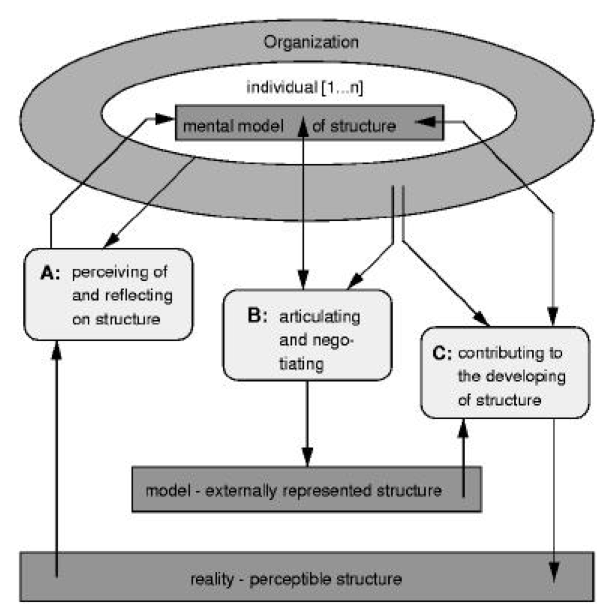
\includegraphics[width=7cm]{img/MentaleModelle/herrmann_levels_of_structure.png}
	\caption[Mentale Modelle im Kontext der Arbeitsmodellierung]{Mentale Modelle im Kontext der Arbeitsmodellierung (entnommen aus \citep{Herrmann02})}
	\label{fig:img_MentaleModelle_herrmann_levels_of_structure}
\end{figure}

\subsubsection{Unterstützung}

Im Rahmen mehrerer Fallstudien zeigen die Autoren, dass die Verwendung von diagrammatischen Modellen als externalisierte Repräsentation von individuellen Sichten auf Arbeitsabläufe bei deren Abstimmung und Verbesserung -- also bei der Durchführung von „Articulation Work“ -- hilfreich ist. Externalisierte Modelle bringen jedoch auch Risiken mit sich, die durch eine adäquate Unterstützung des Modellierungsprozesses gemindert werden müssen. Konkret erwähnen die Autoren die schwierige Veränderbarkeit einmal niedergeschriebener Arbeitsabläufe, die potentiell fehlerhafte oder unzureichende Abbildung des Arbeitsablaufs im Modell sowie (im Kontext der kooperativen Erstellung) jene Unzulänglichkeiten des Modells, die durch bewusst falsch oder nicht offengelegte Arbeitsaspekte aus „politischen“ Gründen entstehen.

\label{steps:herrmann} In der Folge entwickeln \citeauthor{Herrmann02} Anforderungen an einen Modellierungsprozess sowie eine Modellierungssprache, die diese Risiken so weit möglich vermeiden und „Articulation Work“ unterstützen:
\begin{itemize}
	\item Modelle müssen „aus dem Arbeitsablauf heraus“ entstehen, also von den unmittelbar betroffenen Personen entwickelt werden und dürfen nicht von „außerhalb“ übergestülpt werden.
	\item Die Modellierungssprache muss es erlauben, die Dynamik der abgebildeten Strukturen darzustellen.
	\item Sie muss sowohl zur Abbildung (präskriptiver) exakter Arbeitsabläufe („scripts“) als auch zur Abbildung des (Orientierung gebenden) Arbeitskontext („maps“) geeignet sein.
	\item Detaillierungs- und Abstraktionsgrad der Abbildung müssen frei wählbar sein.
	\item Information über den Modellierungsverlauf selbst muss im Modell abbildbar sein.
	\item Die Modellierungssprache muss die Abbildung beliebiger Aspekte von Arbeit (nicht nur Aktivitäten und Ressourcen, sondern z.B. auch Rollen oder Kompetenzen) erlauben.
	\item Der Modellierungsvorgang muss durch ein flexibles Werkzeug unterstützt werden, das die Verwendung der Unterstützungsfunktionalitäten ermöglicht aber nicht erzwingt.
	\item Das Werkzeug sollte den Export der Modelle in beliebige Datenformate ermöglichen, um deren Weiterverarbeitbarkeit zu gewährleisten.
\end{itemize}

\subsubsection{Auswirkungen}

Anhand der Fallstudien zeigen die Autoren, dass das ein Vorgehen nach den beschriebenen Richtlinien, sowie eine entsprechende Werkzeugunterstützung bei der Abstimmung von kooperativen Arbeitsabläufen hilfreich ist (siehe dazu auch \citep{Herrmann00}).

\subsubsection{Bewertung}

Die Arbeit kann als ein Beitrag zur Unterstützung von „Articulation Work“ im Sinne von „making agreements“ verstanden werden, auch wenn dies nicht explizit so benannt wird. In diesem Zusammenhang führen die Autoren die Nützlichkeit von externalisierten Modellrepräsentation bei der Abstimmung und Aushandlung von Arbeitsabläufen an. Für diese Form der Unterstützung werden konkrete Anforderungen sowohl methodischer als auch technischer Natur gegeben, was diese Arbeit zu einer wertvollen Quelle für die weiteren Ausführungen in der vorliegenden Arbeit macht.
\\[1em]
\begin{tabular}{| p{3cm} | p{10cm} |}
  \hline
  Kontext & Modellierung von Arbeit,  \\ \hline
  Art von AW & explizites „agreement making“ \\ \hline
  Unterstützung & flexible Modellierung von Arbeitsabläufen unter Einbeziehung der unmittelbar beteiligten Individuen \\ \hline
  Auswirkungen & Erleichterung bzw. Ermöglichung der Abstimmung oder Aushandlung von kooperativen Arbeitsabläufen \\ \hline
\end{tabular}


\subsection{Recursive Articulation Work in Ariadne: The Alignment of Meanings}
\label{sub:recursive_articulation_work_in_ariadne}

\citep{Sarini02} beschäftigen sich mit „recursive Articulation Work“, also jener Form, deren Gegenstand selbst wiederum „Articulation Work“ ist. Die Autoren leiten Anforderungen an die Unterstützung dieser Form von „Articulation Work“ ab und zeigen die konkrete Umsetzung als Teil des „Reconciler“-Systems.

\subsubsection{Kontext}

Die Arbeit baut auf den oben bereits beschriebenen Arbeiten \citep{Schmidt92} und \citep{Divitini00} auf und beschäftigt sich mit der technischen Unterstützung von „Articulation Work“ durch \gls{CSCW}-Systeme. Konkret wird auf jene Fälle von „Articulation Work“ eingegangen, wo „alignment of meaning“ (also die Abstimmung der individuellen Verständnisse der Arbeitsdomäne) notwendig ist. Es ist kein spezifischer Anwendungsbereich angeführt, das Konzept hat den Anspruch, generisch anwendbar zu sein.

\subsubsection{Unterstützung}

Die Arbeit behandelt zwei unterschiedliche Phasen von „Articulation Work“: jene, in denen die beteiligten Individuen die auftretende Probleme abgrenzen, detailliert spezifizieren und (Teil-)Lösungen aushandeln („agreement making“) und jene, in denen Koordinationsprobleme durch die gesammelte Information bereits vor dem Auftreten verhindert werden („coordination of predefined work“). Während zweitere Unterstützung an dieser Stelle nicht näher behandelt wird, da es sich bei der vorgeschlagenen Implementierung lediglich um ein Vorschlagssystem für Begriffe an der Benutzungsschnittstelle handelt, muss erstere Unterstützungsform näher betrachtet werden.

Der dabei angestoßene Unterstüzungsprozess ist ein Koordinationsmechanismus im Sinne von \citet{Divitini00}. Im Rahmen der Ausführung desselben wird ein „Reconciliation Artifact“ generiert und enthält eine Abbildung der individuellen Begriffswelten der beteiligten Individuen, die untereinander in Korrespondenz gesetzt werden. Wie die Externalisierung der Begriffe, sowie deren Assoziation untereinander ablaufen, schränkt der Ansatz bewusst nicht ein bzw. legt sich nur vorläufig fest\footnote{\emph{„For sake of testing the integration we are aiming at, we defined the simplest protocol: all the users involved in the reconciliation process can communicate among themselves to define the correspondences, while a single Actor assumes the Role of Manager of the Reconciliation Artifact and is in charge of keeping it updated.“}\citep[][S. 10]{Sarini02}}. Das „Reconciler“-System unterstützt dabei die Erfassung und Verwaltung der offengelegten Begriffe. Wie es den Artikulationsprozess konkret unterstützt, ist in \citet{Mark02a} angeführt, hier aber nicht Gegenstand einer detaillierteren Betrachtung, da vorrangig technische Implementierungsdetails beschrieben wurden.

\subsubsection{Auswirkungen}

In der vorliegenden Arbeit werden keine Aussagen hinsichtlich der tatsächlichen Auswirkungen der Unterstützung getroffen. Auch \citet{Mark02a} kommen auf Basis einer empirischen Studie zu dem Schluss, dass die Unterstützungleistung nicht allgemein nachgewiesen werden kann und ist stark von der individuellen Nutzungsbereitschaft abhängig.

\subsubsection{Bewertung}
Die Autoren gehen auf die Unterstützung jenes Teils von „Articulation Work“ ein, der zur Abstimmung der individuellen Sichten auf den Arbeitsablauf und der jeweiligen Begriffswelten eingesetzt wird. Auch wenn sie in der konkreten methodischen Umsetzung vage bleiben, ist erstmals eine explizite Beschäftigung mit der Unterstützung dieser Phase vorhanden.
\\[1em]
\begin{tabular}{| p{3cm} | p{10cm} |}
  \hline
  Kontext & \gls{CSCW} \\ \hline
  Art von AW & explizites „agreement making“, „coordination of predefined work“ \\ \hline
  Unterstützung & durch die Abstimmung der individuellen Sichten auf eine Domäne, der Offenlegung des Vokabulars in einem geteilten Artefakt und dessen Verwendung während der Arbeit \\ \hline
  Auswirkungen & --- \\ \hline
\end{tabular}

\subsection{Combining Communication and Coordination Toward Articulation of Collaborative Activities}

\citet{Raposo04} decken in ihrer Arbeit zur (technischen) Unterstützung kooperativer Arbeit explizit alle Zeitpunkte, in denen „Articulation Work“ auftreten kann, ab („pre-articulation“, „coordination“, „post-articulation“).

\subsubsection{Kontext}

Die Autoren schlagen eine technische Unterstützung von „Articulation Work“ mittels \gls{CSCW}-Werkzeugen vor. Sie fassen dabei das Konzept „Articulation Work“ sehr weit und inkludieren neben der Planungs- und Durchführungsphase eines Arbeitsablaufs auch dessen Nachlauf („post-articulation“), in dem die durchgeführte Koordination reflektiert wird. Zur Unterstützung verfolgen die Autoren einen formalisierten Ansatz, der auf Konzepten der theoretischen Informatik aufbaut. Das Anwendungsgebiet ihres Ansatzes schränken die Autoren nicht ein und berücksichtigen explizit lose wie auch eng gekoppelte kooperative Arbeitsabläufe mit beliebig vielen beteiligten Individuen.

\subsubsection{Unterstützung}

Je nach Phase der „Articulation Work“ unterscheiden die Autoren zwischen unterschiedlichen Arten der Unterstützung. Für die „pre-“ und „post-articulation“-Phase wird die Verwendung von „conversation clichés“ zur Aushandlung von „commitments“ vorgeschlagen. Während der „coordination“-Phase werden die „commitments“ automationsgestützt zur Anwendung gebracht.

„Conversation clichés“ sind im Wesentlichen Zustandsautomaten, die den Rahmen einer Konversation zwischen Individuen vorgeben. Sie dienen jeweils der Erreichung einer bestimmten Art von „commitment“. „Commitments“ sind logische Konstrukte, in denen die individuelle Zustimmung oder Ablehnung zu Aussagen ausgedrückt werden kann, die die Koordination beschreiben. Weiters ist es möglich, explizit kein „commitment“ zu einer Aussage abzugeben. Auf Basis dieser „commitments“ bestimmt ein Algorithmus die Modalitäten der Zusammenarbeit.

Während der „coordination phase“ kommt ein „task/interdependency-model“ zum Einsatz, das im Wesentlichen einem auf die „commitments“ abgestimmten Aktivitätsdiagramm entspricht. In diesem Modell werden letztlich die durchzuführenden Aufgaben und deren gegenseitige Abhängigkeiten definiert. Während der Ausführung kann das System dann auf diese Abhängigkeiten hinweisen bzw. die notwendigen Koordinationsmechanismen auslösen.

\subsubsection{Auswirkungen}

Konkrete Auswirkungen werden in der Publikation nicht angeführt. Die Autoren erwähnen die Simulierbarkeit und Verifizierbarkeit der erstellten Modelle als Vorteil der formalen Repräsentation. 

\subsubsection{Bewertung}
Die Autoren verfolgen einen -- im Gegensatz zu anderen Arbeiten -- stark regulatorischen Ansatz zur Unterstützung von „Articulation Work“. Die vorgeschlagenen Mechanismen zur Abstimmung und Koordination von kooperativer Arbeit versuchen, den Arbeitsverlauf durch computergestützte Vorgaben in einem definierten Rahmen zu halten und so das Auftreten von problematischen Situationen zu verhindern. 

Der Vorteil dieses eher restriktiven Vorgehens liegt in der Formalisierbarkeit der Interaktionsmuster und Arbeitsabläufe und der damit verbundenen Verifizierbarkeit und Simulierbarkeit der erstellten Modelle. 
\\[1em]
\begin{tabular}{| p{3cm} | p{10cm} |}
  \hline
  Kontext & \gls{CSCW}, Formale Modelle von Interaktion \\ \hline
  Art von AW & explizites „making arrangements“, explizite „coordination of predefined work“ \\ \hline
  Unterstützung & \emph{„making arrangements“}: Aushandlungsunterstützung durch „Conversation Clichés“, \emph{„coordination“} durch die Ausführung der ausgehandelten Aufgabenmodelle \\ \hline
  Auswirkungen & formale Verifizierbarkeit und Simulierbarkeit \\ \hline
\end{tabular}

\subsection{Interactive Process Models}
\label{sub:interactive_process_models}

\citet{Jorgensen04} beschreibt die Verwendung von „interaktiven“ Prozessmodellen in organisationalen Arbeitsprozessen und die Veränderung dieser Prozesse durch Modellierungsvorgänge. Dabei bezeichnet er den Modellierungsvorgang als „Articulation Work“.

\subsubsection{Kontext}

Im Gegensatz zu den anderen hier behandelten Arbeiten steht bei \citet{Jorgensen04} nicht die Unterstützung der Koordination von Arbeitsprozessen im Vordergrund. Die Arbeit beschäftigt sich mit Prozessmodellen (also ablauforientierten Modellen von Arbeit) und sieht „Articulation Work“ als jene Tätigkeit, die zur Erstellung dieser Modelle notwendig ist. Die Rückwirkung der Modelle auf die reale Arbeitswelt wird als „Model Activation“ bezeichnet. Modellierung ist hierbei eine Aktivität, die von den betroffenen Personen selbst ausgeführt wird, die erstellten Modelle bilden dementsprechend die individuelle Sicht auf eine Arbeitsablauf ab. Insofern ist der vorgestellt Ansatz tatsächlich als eine Form von „making arrangements“ (als Variante von expliziter, planender „Articulation Work“) zu sehen.

\subsubsection{Unterstützung}

\citeauthor{Jorgensen04} führt Anforderungen an eine Modellierungssprache an, die „Articulation Work“ unterstützt. \label{steps:jorgensen} Diese sollte:
\begin{itemize}
	\item einfach sein und nur wenige Basiselemente enthalten. Elemente der realen Welt sollten eindeutig in das Modell abgebildet werden können. Die Aussage des Modells sollte möglichst intuitiv erschließbar sein.
	\item visuell bzw. graphisch darstellbar sein. Die Darstellung sollte sowohl einen Überblick über das Gesamtmodell als auch detaillierte an sichten einzelner Ausschnitte ermöglichen.
	\item Konstrukte enthalten, die auf die jeweilige Anwendungsdomäne der Modellierenden abgebildet bzw. angepasst werden können.
	\item nicht statisch hinsichtlich der Bedeutung der verwendeten Modellelemente sein. Die Bedeutung der Modellelemente kann sich während der Erstellung der Modelle durch Aushandlung oder Reflexion verändern.
\end{itemize}

Der Autor führt zur Erfüllung dieser Anforderungen eine Modellierungssprache ein, die den Ansatz des „semantic holism“ verfolgt. In Sprachen, die den Ansatz des „semantischen Holismus“ berücksichtigen, haben Modellelemente keine eindeutige, fix vorgegebenen Bedeutung. Vielmehr erschließt sich der Bedeutung der einzelnen Elemente erst aus dem Gesamtzusammenhang des Modells, also aus dem Zusammenspiel aller Elemente.

Auch im Feld der „coordination of predefined work“ liefert \citet{Jorgensen04} Ansätze zur Unterstützung von Articulation Work, indem er die erstellten Modelle semi-automatisiert („interactive“) ausführbar macht („activation“).

\subsubsection{Auswirkungen}

Der Autor führt keine konkrete Evaluierung seines Ansatzes an, weshalb keine Aussagen zu den Auswirkungen des Ansatzes in der Praxis gemacht werden können. Aus der zugrunde liegenden Literatur leitet er jedoch ab, dass der gewählte Ansatz zur Modellierung eine adäquatere und einfachere Abbildung der Realität durch in der Modellierung ungeübte Individuen ermöglicht als andere gängige Modellierungs-Methoden.

\subsubsection{Bewertung}
Die Fokussierung auf Modellbildung als Aktivität im Rahmen von „Articulation Work“ ist ein Alleinstellungsmerkmal dieser Arbeit. \citeauthor{Jorgensen04} berücksichtigt die für „Articulation Work“ notwendige Flexibilität in der technischen und methodischen Unterstützung derselben und stellt Anforderungen auf, die eine Modellierungssprache erfüllen muss, um „Articulation Work“ adäquat zu unterstützen. Die Unterstützung der Ausführung der Modelle in interaktiver Form ohne die im \gls{WfMS} üblichen strikten Abläufe kommt einer flexiblen Koordination des eigentlichen Arbeitsablaufs ebenfalls entgegegen.
\\[1em]
\begin{tabular}{| p{3cm} | p{10cm} |}
  \hline
  Kontext & Prozessmodellierung, Workflow-Managment \\ \hline
  Art von AW & explizites „making arrangements“, „coordinating predefined work“ \\ \hline
  Unterstützung & \emph{„making arrangements“}: durch flexible, anwenderzentrierte Modellbildung, \emph{„coordinating“}: durch interaktive Ausführung der erstellten Modelle \\ \hline
  Auswirkungen & adäquate und einfache Abbildung sowie intuitive Interpretierbarkeit der Modelle und damit Unterstützung von expliziter „Articulation Work“ durch Modelle von Arbeit \\ \hline
\end{tabular}

\subsection{Torres, a Conceptual Framework for Articulation Work across Boundaries}

\citet{Cabitza06} stellen mit „Torres“ ein Framework vor, das sich speziell zur Unterstützung von „globaler Articulation Work“ eignet.

\subsubsection{Kontext}

\citet{Cabitza06} entwickeln den weiter oben beschriebenen Ansatz von \citet{Sarini02} weiter und wenden ihn unter Bezugnahme auf \citet{Faergemann05} auf „globale Articulation Work“ an. Die Autoren stehen damit in der Tradition der technischen Unterstützung von „Articulation Work“ durch \gls{CSCW}-Werkzeuge und wenden diese im speziellen auf Situationen an, in denen Individuen oder Organisationseinheiten kooperieren müssen, die außerhalb des betreffenden Arbeitsablaufs keine kooperativen Tätigkeiten durchführen.

\subsubsection{Unterstützung}

Die Autoren bleiben grundsätzlich bei dem Ansatz von \citet{Sarini02}, die Koordination von Arbeit mittels Artefakten zu unterstützten, die auf den jeweiligen Anwendungsfall angepasst sind. „Torres“ ist dabei ein Framework zur Erstellung derartiger Artefakte. \label{steps:cabitza} Dazu wird ein zweistufiger Prozess vorgeschlagen, der die domänenübergreifende Verständlichkeit der artikulierten Information sicherstellen soll.

In der ersten Phase werden von jedem beteiligten Individuum bzw. von jeder beteiligten Instanz „Local Formal Representations“ der jeweiligen Domäne erstellt werden. Diese enthalten nicht Modelle der Arbeitsabläufe selbst sondern lediglich die wesentlichen Konzepte der Domäne, die potentiell missverständlich sein können.

In der zweiten Phase werden die „Local Formal Representations“ zu einem einheitlichen, vorgegebenen Modell von „Articulation Work“ mittels ebenfalls vorgegebener Relationen in Beziehung gesetzt. Dadurch ist es möglich, etwaig auftretende Missverständnisse automationsgestützt aufzulösen bzw. zu vermeiden.

\subsubsection{Auswirkungen}

Die Autoren leiten die Eigenschaften ihres Systems aus den Beobachtungen in einer Fallstudie aus dem medizinischen Bereich ab. Die Implementierung war jedoch zum Zeitpunkt der Publikation nicht abgeschlossen, auch in Folgepublikationen (z.B. \citep{Cabitza09b}) ist keine explizite Beschreibung von Auswirkungen des Systems im praktischen Einsatz vorhanden.

\subsubsection{Bewertung}
Die Autoren entwickeln den in \citet{Sarini02} vorgeschlagenen „Reconciler“-Ansatz weiter und detaillieren vor allem jene Phase, in der „alignment of meanings“ durchgeführt wird. Methodisch schlagen die Autoren einen individuell durchzuführende zweistufigen Prozess vor, dessen Ergebnisse automatisiert mit den Ergebnissen der anderen Individuen zusammengeführt werden. Methodisch ist dies der detaillierteste Ansatz der Arbeiten der Gruppe rund um Simone und wird deswegen an dieser Stelle betrachtet.
\\[1em]
\begin{tabular}{| p{3cm} | p{10cm} |}
  \hline
  Kontext & \gls{CSCW} \\ \hline
  Art von AW & „making arrangements“ \\ \hline
  Unterstützung & \emph{methodisch:} Abstimmung unterschiedlicher Domänenmodelle und Erstellung von Informations-Artefakten, die domänenübergreifend verständlich sind \\ \hline
  Auswirkungen & --- \\ \hline
\end{tabular}

\subsection{Gegenüberstellung und Zusammenfassung} % (fold)
\label{sub:gegenüberstellung_und_zusammenfassung}

Die Möglichkeiten zur Unterstützung von „Articulation Work“ sind ob der großen Spannweite möglicher Ausprägungen vielfältig. Im Allgemeinen zeigt sich die Tendenz, dass die Unterstützung bei einfacheren Formen (wie „coordination of predefined work“) eher mittels rein organisationalen Mitteln erfolgen kann, während bei komplexeren Formen von „Articulation Work“ zusätzlich auch technische Mittel eingesetzt werden und methodische Unterstützung angeboten wird. Außerdem soll durch technische Unterstützung der Phase, die dem eigentlichen Arbeitsablauf voraus geht (Planung, „making original arrangements“) das Auftreten von problematischen Situationen (und damit der Bedarf nach komplexen Formen von „Articulation Work“) während der Durchführung des Arbeitsablaufs vermieden werden.

Für einfache Formen von „Articulation Work“, in denen etablierte Arbeitsabläufe koordiniert bzw. kleine Unklarheiten oder Hindernisse beseitigt werden müssen, werden in der Literatur immer wieder soziale Mechanismen als ausreichendes Regulativ beschrieben (z.B. in \citep{Raposo01} oder \citep{Schmidt94}). \citet{Davenport02} nennt „Communities of Practice“ \citep{Wenger99} als mögliches Instrument zur Institutionalisierung dieser sozialen Mechanismen. Einen Spezialfall stellen hier jene Arbeitsabläufe dar, die verteilt durchgeführt werden und in denen deshalb die sozialen Mechanismen durch technische Mittel ermöglicht werden müssen \citep{Faergemann05}. In diesen Fällen werden auch einfache Formen von „Articulation Work“ technisch unterstützt (z.B. bei \citep{Divitini00} oder \citep{Fuchs01}).

Je komplexer die Arbeitssituation wahrgenommen wird, desto notwendiger wird eine explizite Beschäftigung mit den abzustimmenden Arbeitsaspekten (auch bei Arbeitsabläufen, die nicht oder nur in Teilaspekten kooperativ bearbeitet werden \citep{Fjuk97}). Letztendliches Ziel ist es immer, einen Status (wieder-)herzustellen, in dem soziale, implizite Mechanismen zur Koordination ausreichen. Organisationale (z.B. bei \citep{Grinter96}) oder auch technische Unterstützung (z.B. bei \citep{Schmidt00} und allen auf dieser Publikation aufbauenden Arbeiten) kann hierbei hilfreich sein.

Bei der technischen Unterstützung von „Articulation Work“ können zwei Ansatzpunkte unterschieden werden. Einerseits kann die Lösung von aufgetretenen Problemen unterstützt werden (z.B. bei \citep{Grinter96}) oder deren Auftreten von vorneherein verhindert werden (z.B. bei \citep{Raposo04}). Andererseits kann „Articulation Work“ bei der Planung von Arbeitsprozessen unterstützt werden, wobei unter anderem die Koordinationsmechanismen während der Durchführung des Arbeitsablaufs vereinbart werden (z.B. bei \citet{Sarini02a} und den darauf aufbauenden Arbeiten). Ziel ist es hier, schon im Vorfeld den Arbeitsablauf bzw. die unterschiedlichen Sichten darauf soweit abzustimmen, dass die Koordination möglichst unproblematisch und implizit abgehandelt werden kann.

Diese Form von „Articulation Work“ wird vom Großteil der in diesem Bereich tätigen Autoren durch Modelle der zu koordinierenden Arbeit als explizite Artefakte im Artikulationsprozess unterstützt (z.B. bei \citep{Divitini00}, \citep{Sarini02}, \citep{Raposo04} oder \citep{Jorgensen04}). Diese Modelle werden von den beteiligten Personen erstellt und müssen syntaktisch einfach bzw. intuitiv zu handhaben und semantisch flexibel sein \citep{Herrmann02} \citep{Jorgensen04}. Der Inhalt der Modelle kann sowohl der eigentliche Arbeitsablauf sein \citep{Divitini00} als auch die allgemeinen Struktur der Arbeitsdomäne konzeptuell abbilden \citep{Sarini02}. 

Die existierenden Arbeiten in diesem Bereich setzten allerdings die Existenz dieser Modelle voraus bzw. schaffen die konzeptuellen Rahmenbedingungen, um die Erstellung derartiger Modelle zu ermöglichen. Dabei sind sie immer durch den Anspruch eingeschränkt, die Modelle automationsgestützt zur Unterstützung der Koordination im Arbeitsablauf selbst weiterzuverarbeiten. Die Anforderung an die Modellierungssprache sind also nur zum Teil aus den Bedürfnissen der Benutzer abgeleitet, sondern vielmehr ein Kompromiss zwischen den Anforderungen des technischen Systems und der Bedürfnisse der Benutzer. Mit der konkreten Erstellung der Modelle selbst beschäftigen sich lediglich \citet{Herrmann02} sowie \citet{Jorgensen04}, auch sie gehen aber nicht auf die konkrete Unterstützung der Individuen im Modellierungsprozess ein.

Die Unterstützung der an einem Arbeitsablauf beteiligten Individuen bei Modellbildung und -abstimmung als „Articulation Work“ weist an dieser Stelle also Lücken auf, die bislang nicht behandelt wurden. Dies ist insofern problematisch, als dass vor allem komplexe Formen von „Articulation Work“ auf externe Repräsentationen zurückgreifen, um die Abstimmung zu erleichtern. Im weiteren Verlauf dieser Arbeit wird deswegen versucht, methodische und technische Hilfsmittel zu entwickeln, die auf Modellen basierende „Articulation Work“ unterstützen kann. Einen möglichen Ansatzpunkt dazu liefert bereits \citet{Strauss93}.

% subsection gegenüberstellung_und_zusammenfassung

% section unterstützung_von_articulation_work (end)

\section{Thought processes und Articulation Work} % (fold)
\label{sec:aw_fazit}

Zur Zielsetzung von „Articulation Work“ und deren Unterstützung treffen die im letzten Abschnitt betrachteten Arbeiten klare Aussagen. Offen bleiben jedoch vor allem bei der Unterstützung komplexerer Formen von „Articulation Work“ explizite Aussagen zu den notwendigen Leistungen der Individuen im Prozess der Artikulation, deren konkrete Ausgestaltung und der möglichen Unterstützung. 

Bereits Strauss ist sich dieser (konzeptuellen) Auslassung bewusst\footnote{\emph{„[\ldots] many social scientist pay almost no attention to interior activity: ignoring it, taking it for granted, but leaving it unexamined, or giving it the kind of abstract but not very detailed analysis [\ldots]“}\citep[][S. 131]{Strauss93}}, und beschäftigt sich in späteren Arbeiten (etwa \citep{Strauss93}) auch mit jenen kognitiven Vorgängen, die von ihm als „thought processes“ oder „mental activities“ bezeichnet werden und die untrennbar mit jeder Art von Tätigkeit und Interaktion verbunden sind\footnote{\emph{„These [thought processes] accompany visible action, as well as precede and follow in conditional and consequential modes“}\citep[][S. 146]{Strauss93}} und diese beeinflussen\footnote{\emph{„Even well-grooved, routine action and interaction may be accompanied by thought [\ldots] directly relevant to the work at hand. As I vacuum the house, barely noticing my movements, still I give myself commands [\ldots]“}\citep[][S. 132]{Strauss93}}. 

Im Kontext der Abstimmung von Arbeitsabläufen kommt den „thought processes“ der Individuen große Bedeutung zu, da sie den sichtbaren individuellen Handlungen zugrunde liegen bzw. diese beeinflussen. „Articulation Work“ wirkt sich also auf die „thought processes“ der beteiligten Individuen aus (wie auch von \citet{Davenport02} im Kontext des „situated learning“ erwähnt). Strauss interessiert sich allerdings ausschließlich für die dynamischen Aspekte der Interaktion zwischen Individuen, nicht aber für die Ausgangspunkte und Ergebnisse der zugrunde liegenden „thought processes“.\footnote{\emph{„I use the gerund 'ing' after 'symbol' [bei der Beschreibung von 'symbolizing', Anm.] to signify that my principal interest is, again, in interaction rather than its products, for symbols are precipitates of interaction“}\citep[][S. 149]{Strauss93}} 

Die Repräsentationen, auf denen „thought processes“ beruhen und operieren, sind jedoch für die Unterstützung von „Articulation Work“ von Interesse. Vorhandene Arbeiten (etwa \citep{Herrmann02} oder \citep{Jorgensen04}) beschäftigen sich lediglich mit bereits externalisierten Repräsentationen, gehen jedoch ebenfalls nicht auf deren Erstellung oder Ursprung ein. Die kognitions-wissenschaftlichen Ansätze zu Schemata (\citep{Rumelhart78} \citep[vgl. nach ][]{Hanke06}) und mentalen Modellen (\citep[vgl. ][]{Seel91}) sind ein Erklärungsansatz für diese Lücke \citep{Herrmann02}.

% section fazit (end)

\section{Zusammenfassung} % (fold)
\label{sec:aw_zusammenfassung}

In diesem Abschnitt wurde „Articulation Work“ als ein Erklärungsmodell für die koordinierenden Abläufe bei kooperativer menschlicher Arbeit eingeführt. Nach einer Begriffsklärung auf Basis der zur Thematik publizierten Literatur wurden die unterschiedlichen Ausprägungen beschrieben, in denen „Articulation Work“ auftreten kann und in welchen Situationen welche Ausprägung auftritt. Den Abschluss des allgemeinen Teils bildet eine Übersicht über die Gegenstände von „Articulation Work“, also jene Arbeitsaspekte, die potentiell abgestimmt werden müssen.

Der zweite Teil des Kapitels beschreibt technische und methodische Möglichkeiten zur Unterstützung der Durchführung von „Articulation Work“. Die dort identifizierten Ansätze zeigen ein breites Spektrum von Möglichkeiten der Unterstützung für unterschiedliche Ausprägungen von „Articulation Work“. Vor allem im Bereich der Unterstützung von „explizter Aritculation Work“, also der bewusst angestossenen und durchgeführten Form von „Articulation Work“, kommen in einem Großteil der Arbeiten diagrammatische Modelle zum Einsatz. Diese erleichtern die Abstimmung und ermöglichen die einfacherer und schnellere Entwicklung einer gemeinsamen Sichtweise auf den betrachteten Arbeitsablauf.

\subsection{Beitrag zur globalen Zielsetzung}

Hinsichtlich der in Kapitel \ref{cha:einführung} formulierten Forschungsfragen und Fragestellungen wurde in diesem Kaptitel vor allem die Fragestellung \ref{tf:was_is_aw} („Was ist Articulation Work und wie wirkt sie im Arbeitsprozess“) behandelt. Die relevanten Konzepte und Untersuchungen wurden in den Abschnitten \ref{sec:aw_begriffsbestimmung} und \ref{sec:arten_von_articulation_work} erarbeitet und einander gegenübergestellt (auf Grundlage der in Anhang \ref{cha:literatur_zum_themengebiet_articulation_work} aufgearbeiteten Literatur zum Themengebiet „Articulation Work“). Das Ergebnis der Aufarbeitung ist eine Konzeption von „Articulation Work“, in der alle in der Literatur genannten Auslöser, Ausprägungen und Zielsetzungen berücksichtigt wurden (siehe Abbildung \ref{fig:img_ArticulationWork_aw_conceptual_structure}). 

In Abschnitt \ref{sec:abzustimmende_arbeitsaspekte} wurde mit der Betrachtung der im Rahmen von „Articulation Work“ abzustimmenden Aspekte der „Production Work“ jene Betrachtungsgegenstände identifiziert, an denen sich die Durchführung von „Articulation Work“ zeigt. Für diese Arbeit ist dies von Interesse, als dass an diesen die Effektivität der Durchführung von „Articulation Work“ beobachtet werden kann. Diese Effektivität ist dann gegeben, wenn eine gemeinsame Sichtweise auf die abzustimmenden Gegenstände, konkret also die relevanten Aspekte des Arbeitsablaufs selbst sowie jene aus dessen Umfeld, entwickelt wurde. Dies ist ein erster Beitrag zur Bearbeitung der Fragestellung \ref{tf:beurteilung_der_effektivität} („Wie kann die Effektivität der Unterstützung von expliziter Articulation Work beurteilt werden?“).

Die in Abschnitt \ref{sec:unterstützung_von_articulation_work} dargestellte Literatur zum Themengebiet der Unterstützung von „Articulation Work“ konkretisiert einerseits die Beantwortung der Fragestellung \ref{tf:was_is_aw} hinsichtlich der Wirkungsweise in Arbeitsprozessen, trägt aber andererseits vor allem zur Erarbeitung der Möglichkeiten zur methodischen Unterstützung von „Articulation Work“ bei (Fragestellung \ref{tf:methoden}). Auf Basis der dortigen Ergebnisse zeigt sich, wie in Abschnitt \ref{sub:gegenüberstellung_und_zusammenfassung} beschrieben, dass in existierenden Arbeiten zur Unterstützung von „Articulation Work“ nur auf die zu unterstützenden Phänomene und Abläufe eingegangen wurde. Die zweite von \citet{Grudin88} formulierte Forderung nach einer Berücksichtigung der Bedürfnisse und Tätigkeiten der beteiligten Individuen (siehe Kapitel \ref{cha:einführung}) wurde bislang nicht behandelt. Abschnitt \ref{sec:aw_fazit} weist auf einen möglichen Ansatzpunkt hin, die Fragestellung \ref{tf:methoden} im Sinne von \citet{Grudin88} vollständiger bearbeiten zu können.

\subsection{Weitere Verwendung der Ergebnisse}

Die zur Unterstützung von „Articulation Work“ von mehreren Autoren vorgeschlagene Erstellung von diagrammatischen Modelle wird in existierenden Arbeiten methodisch nur teilweise behandelt. Vor allem die Rolle der beteiligten Individuen und deren Unterstützung im Erstellungsprozess bleibt unklar. Dies ist insofern problematisch, als dass die erfolgreiche Durchführung von „Articulation Work“ die Einbindung aller beteiligten Individuen bedingt und deren Sichtweise auf den abzustimmenden Arbeitsablauf berücksichtigen muss. Als Ansatzpunkt, die Berücksichtigung dieser individuellen Beiträge bei der Durchführung von „Articulation Work“ sicherzustellen und methodisch sowie mit einem Werkzeug zu unterstützen, wurde das Konzept der „Mentalen Modelle“ als geeignet identifiziert. In Kapitel \ref{cha:mentale_modelle} werden diese nun konzeptuell eingeführt und hinsichtlich der Anforderungen im Rahmen der Durchführung von „Articulation Work“ betrachtet.

% section zusammenfassung (end)
% chapter articulation_work (end)

